% mnras_template.tex 
%
% LaTeX template for creating an MNRAS paper
%
% v3.0 released 14 May 2015
% (version numbers match those of mnras.cls)
%
% Copyright (C) Royal Astronomical Society 2015
% Authors:
% Keith T. Smith (Royal Astronomical Society)

% Change log
%
% v3.0 May 2015
%    Renamed to match the new package name
%    Version number matches mnras.cls
%    A few minor tweaks to wording
% v1.0 September 2013
%    Beta testing only - never publicly released
%    First version: a simple (ish) template for creating an MNRAS paper

%%%%%%%%%%%%%%%%%%%%%%%%%%%%%%%%%%%%%%%%%%%%%%%%%%
% Basic setup. Most papers should leave these options alone.
\documentclass[fleqn,usenatbib]{mnras}

% MNRAS is set in Times font. If you don't have this installed (most LaTeX
% installations will be fine) or prefer the old Computer Modern fonts, comment
% out the following line
\usepackage{newtxtext,newtxmath}
% Depending on your LaTeX fonts installation, you might get better results with one of these:
%\usepackage{mathptmx}
%\usepackage{txfonts}

% Use vector fonts, so it zooms properly in on-screen viewing software
% Don't change these lines unless you know what you are doing
\usepackage[T1]{fontenc}
\usepackage{ae,aecompl}




%%%%% AUTHORS - PLACE YOUR OWN PACKAGES HERE %%%%%

% Only include extra packages if you really need them. Common packages are:
\usepackage{graphicx}	% Including figure files
\usepackage{amsmath}	% Advanced maths commands
\usepackage{amssymb}	% Extra maths symbols
\usepackage{siunitx} %v. useful units package 

%%%%%%%%%%%%%%%%%%%%%%%%%%%%%%%%%%%%%%%%%%%%%%%%%%

%%%%% AUTHORS - PLACE YOUR OWN COMMANDS HERE %%%%%

% Please keep new commands to a minimum, and use \newcommand not \def to avoid
% overwriting existing commands. Example:
%\newcommand{\pcm}{\,cm$^{-2}$}	% per cm-squared
\newcommand{\xip}{\ensuremath{\xi_{+}}}
\newcommand{\xim}{\ensuremath{\xi_{-}}}
\newcommand{\xipm}{\ensuremath{\xi_{\pm}}}
\newcommand{\gammat}{\ensuremath{\gamma_{t}(\theta)} }
\newcommand{\wtheta}{\ensuremath{w(\theta)} }
\newcommand{\dsigr}{\ensuremath{\Delta\Sigma(R)}}
\newcommand{\dsigobsr}{\ensuremath{\Delta\Sigma^{\mathrm{obs}}(R)}}
\newcommand{\dsigmodr}{\ensuremath{\Delta\Sigma^{\mathrm{model}}(R)}}

\newcommand{\pgg}{\ensuremath{P_{\mathrm{gg}}}}
\newcommand{\pgm}{\ensuremath{P_{\mathrm{gm}}}}
\newcommand{\xigg}{\ensuremath{\xi_{\mathrm{gg}}}}
\newcommand{\xigm}{\ensuremath{\xi_{\mathrm{gm}}}}




%units
\DeclareSIUnit \megaparsec {Mpc}
\DeclareSIUnit \h {\mbox{$h$}}

%cosmo parameters
\newcommand{\om}{\ensuremath{\Omega_{\mathrm m}}}
\newcommand{\ol}{\Omega_{\mathrm \Lambda}}
\newcommand{\omb}{\Omega_{\mathrm b}}
\newcommand{\sig}{\ensuremath{\sigma_8}}
\newcommand{\lcdm}{$\Lambda$CDM}
\newcommand{\wcdm}{$w$CDM}
\newcommand{\ns}{n_s}
\newcommand{\w}{w_0}
\newcommand{\wa}{w_a}

% eqn and figures
\newcommand\eqn[1]{equation~\ref{#1}}
\newcommand\eqnb[2]{equations~\ref{#1}~\& \ref{#2}}
\newcommand\eqnc[2]{equations~\ref{#1}--\ref{#2}}
\newcommand\Eqn[1]{Equation~\ref{#1}}   % If you need to start a sentence with this...
\newcommand\Eqnb[2]{Equations~\ref{#1}~\& \ref{#2}}

% Likewise for figures and tables
\newcommand\fig[1]{Figure~\ref{#1}}
\newcommand\figb[2]{Figures~\ref{#1}~\& \ref{#2}}
\newcommand\chap[1]{Chapter~\ref{#1}}
\newcommand\sect[1]{Section~\ref{#1}}
\newcommand\tab[1]{Table~\ref{#1}}
\newcommand\app[1]{Appendix~\ref{#1}}
\newcommand{\redmagic}{\texttt{redMaGiC}\,}
\newcommand{\mice}{\texttt{MICE}\,}
\newcommand{\maglim}{\texttt{Maglim}\,}
\newcommand{\buzzard}{\texttt{Buzzard}\,}

\newcommand{\SP}[1]{{\color{brown}[SP: #1]}}
\newcommand{\brown}[1]{\textcolor{brown}{#1}}

%%%%%%%%%%%%%%%%%%%%%%%%%%%%%%%%%%%%%%%%%%%%%%%%%%

%%%%%%%%%%%%%%%%%%% TITLE PAGE %%%%%%%%%%%%%%%%%%%

% Title of the paper, and the short title which is used in the headers.
% Keep the title short and informative.
\title[Short title, max. 45 characters]{DES Y3 results: Constraints on cosmological parameters and galaxy bias models from galaxy clustering and galaxy-galaxy lensing}

% The list of authors, and the short list which is used in the headers.
% If you need two or more lines of authors, add an extra line using \newauthor
\author[DES et al.]{
DES
}

% These dates will be filled out by the publisher
\date{Accepted XXX. Received YYY; in original form ZZZ}

% Enter the current year, for the copyright statements etc.
\pubyear{2015}

% Don't change these lines
\begin{document}
\label{firstpage}
\pagerange{\pageref{firstpage}--\pageref{lastpage}}
\maketitle

% Abstract of the paper
\begin{abstract}
We present cosmological constraints from the combination of galaxy clustering and galaxy-galaxy lensing measurements from the DES Y3 data. We describe our modeling framework and choice of scales, validating their robustness to small-scale theoretical uncertainties by analysing simulated data. We implement nonlinear bias models that include parameterizations based on Lagrangian perturbation theory. We present cosmological constraints when using various (coupled) choices of scale cuts and bias models and demonstrate stability of the constraints. We reproduce the baseline choices of the 3x2 cosmology paper, and consider additional choices that make use of small scale information.  Combining with external datasets including Planck, we show constraints on w, as well as higher order galaxy bias parameters
\end{abstract}

% Select between one and six entries from the list of approved keywords.
% Don't make up new ones.
\begin{keywords}
keyword1 -- keyword2 -- keyword3
\end{keywords}

%%%%%%%%%%%%%%%%%%%%%%%%%%%%%%%%%%%%%%%%%%%%%%%%%%

%%%%%%%%%%%%%%%%% BODY OF PAPER %%%%%%%%%%%%%%%%%%

\section{Introduction}
\label{sec:intro}
\begin{itemize}
    \item LSS can tell us about dark energy.
    \item Galaxy clustering and galaxy-galaxy lensing is a good combo for probing LSS.
    \item Modeling galaxy bias is the main theoretical challenge for this.
\end{itemize}

Wide area imaging surveys of galaxies provide cosmological information through measurements of galaxy clustering and weak gravitational lensing. In recent years, two-point correlations and cross-correlations of the galaxy positions and lensing shear have been used to constrain cosmological parameters in the late time universe. The Dark Energy Survey (DES) analyzed the lensing two-point correlation (cosmic shear) and all three two-point correlations from its Year 1 (Y1) dataset in separate papers. 

The relationship of galaxies to the mass distribution, called galaxy bias, has been a limiting factor in interpreting the galaxy autocorrelation function (denoted) $w(\theta)$) and the galaxy-shear cross-correlation, also called galaxy-galaxy lensing (and denoted $\gamma_t(\theta)$). At large scales, galaxy bias can be described by a single number, the linear bias $b_1$. On smaller scales bias is nonlocal and nonlinear and its description is complicated. Perturbation theory (PT) approaches have been developed for quasilinear scales $\sim 10$ Mpc, though the precise range of scales of its validity is a subtle question that depends on the galaxy population, the theoretical model and the statistical power of the survey. 

With a model for galaxy bias, $w(\theta)$ and $\gamma_t$ measurements, called the ``2x2'' datavector,   can probe the underlying matter power spectrum. They are also sensitive to the distance-redshift relation over the redshift range of the lens and source galaxy distributions.  These two datavectors constitute a useful subset of the full ``3x2'' datavector, which includes cosmic shear, since bias and cosmological parameters can both be constrained (though either $w(\theta)$ or $\gamma_t(\theta)$ individually would be limited by the uncertainty in galaxy bias). 

PT models of galaxy bias are validated using mock catalogs based on N-body simulations with various schemes of populating galaxies. The halo occupation distribution (HOD) approach has been widely developed and is used for the DES galaxy samples. For the Year 3 (Y3) dataset of DES, two independent sets of mock catalogs have been developed, basd on the \buzzard and \mice simulations. 

In this study, we will use PT models for galaxy bias, validate them with mock catalogs and carry out a cosmological analysis of the DES Y3 $w(\theta)$ and $\gamma_t$ measurements.




\section{Statistics and theory}
\label{sec:stat_theory}
\subsection{Two-point statistics}
\label{sec:2pt}
\begin{itemize}
    \item Describe the statistics we use, \wtheta\ and \gammat.
    \item Show their relation to the underlying 3d correlation functions $\xigg(r)$ and $\xigm(r)$
\end{itemize}

\brown{Using the catalog of the positions of foreground lens galaxies and the catalog of shape and positions of background source galaxies, one can construct three two point summary statistics. The two point auto-correlation of the positions of lens galaxies (galaxy clustering), auto-correlation of the lensing shear estimated from shape of background source galaxies (cosmic shear) and  cross-correlation of this lensing shear field and position of lens galaxies (galaxy-galaxy lensing). 

For the galaxy clustering we use the $w(\theta)$ statistic which quantifies the average excess number of galaxy pairs at a separation $\theta$ over a random distribution. For galaxy-galaxy lensing, we use the statistic of $\gamma_{\rm t}(\theta)$ that describes the average tangential component of the shear with respect to the lens-source separation direction. For cosmic shear, which is a spin-2 field, we use the statistic of $\xi_{+}$ and $\xi_{-}$. }


\subsection{P(k) predictions}
\label{sec:Pk_pred}
\begin{itemize}
    \item Heavily referencing the 3D bias paper, describe range of perturbation theory models for $\xigg(r)$ and $\xigm(r)$ and their expected scales of applicability. 
    \item To aid discussion, include some plots showing the sensitivity of our statistics to scales in $\xigg(r)$ and $\xigm(r)$.
    
    \brown{As we saw in the previous section, the statistics of our main interest here $w(\theta)$ and $\gammat$ is related to the underlying 3D correlation functions \xigg and \xigm respectively. }
    
\end{itemize}

\subsection{The rest of the model}
\label{sec:full_pk_th}
Describe the rest of the modelling framework:
\begin{itemize}
    \item IAs (NLA)\brown{TATT?}
    \brown{Galaxy galaxy lensing aims to isolate the percent-level coherent shape distortions, or shear, of background source galaxies due to graviataional field of foreground lens galaxies. However, the local environment can align the source galaxies as well as also contribute to the shear signal through lensing distortions. Since this interaction between the source galaxies and their local environment is non-random, it has non-zero contribution to the galaxy-galaxy lensing signal which we need to model. In this analysis we follow the mixed alignment methodolgy of \cite{Blazek_2019}. }
    \item Magnification
    \brown{All the matter between observed galaxy and the observer acts as a gravitational lens. Hence the galaxies get magnified which results in an increase in the size of galaxy images as well as increase in their total flux. The increase in the size of galaxies results in decrease in observed number density (due to stretching of local sky), whereas due to increase in total flux results in increase in number density (as intrinsically fainter galaxies, which are more numerous, can be observed).  }
    \item RSD
    \brown{}
\end{itemize}    

    
    \SP{
    \begin{itemize}
    \item Point-mass marginalization 
    \item  Motivate that we will be using the $\Sigma^{-1}_{\rm crit}$ factors when doing the PM marginalization. 
    \item \textbf{\textit{Figure}} Plot comparing the contours with vs without PM marginalization for both 2x2pt and 3x2pt. Make (or show) the argument that it is because of breaking of degeneracy between PM and S8. Basically make the case that PM does not matter for 3x2pt and that 2x2pt can have more aggressive scale cuts than 3x2pt analysis.
    \end{itemize}
    }
    
        
    \brown{The galaxy-galaxy lensing signal is related to the mass density of lenses by:
    \begin{equation}
        \gamma_{\rm t}(R;z_{\rm l},z_{\rm s}) = \frac{\Delta \Sigma (R;z_{\rm l})}{\Sigma_{\rm crit} (z_{\rm l},z_{\rm s})},
    \end{equation}
    where, $\Delta \Sigma(R;z_{\rm l}) = \bar{\Sigma}(0,R; z_{\rm l}) - \Sigma(R;z_{\rm l})$ and $\Sigma(R;z_{\rm l})$ is the surface mass density at a transverse separation $R$ from the lens at redshift $z_{\rm l}$ and $\bar{\Sigma}(0,R)$ is the average surface mass density within a separation $R$ from that lens. Through $\bar{\Sigma}(0,R)$ term, $\gamma_{\rm t}$  at any scale $R$, is dependent on mass distribution at all scales less than $R$. This makes $\gamma_{\rm t}$ statistic highly non-local and any model that is valid only on large scales above some $r_{\rm min}$ (like PT) will break down more rapidly than for a more local statistic like \wtheta. However, as the dependence on small scales is through the \textit{mean} surface mass density, the impact of mass distribution inside $r_{\rm min}$ on \gammat can be written as:
    \begin{equation}
        \gamma_{\rm t}(R;z_{\rm l},z_{\rm s}) = \frac{1}{\Sigma_{\rm crit}(z_{\rm l},z_{\rm s})} \bigg(\Delta \Sigma^{\rm model}(z_{\rm l}) + \frac{B(z_{\rm l})}{R^2} \bigg),
    \end{equation}
    where, $\Delta \Sigma^{\rm model}$ is the prediction from a model that is valid of scales above $r_{\rm min}$ and $B$ is the effective total mass below $r_{\rm min}$.  The average $\gamma_{\rm t}$ signal between lens bin $i$ and source bin $j$ can be written as:
    \begin{equation}
        \gamma_{{\rm t},ij} = \gamma^{\rm model}_{{\rm t},ij} + C_{ij}/\theta^2,
    \end{equation}
    where,
    
    \begin{equation}\label{eq:pm_Cij}
        C_{ij} = \int dz_{\rm l} \ dz_{\rm s} \ n_{{\rm l},i} \ n_{{\rm s},j} \ B_i(z_{\rm l}) \ \Sigma^{-1}_{\rm crit}(z_{\rm l},z_{\rm s}) \ \chi^{-2}(z_{\rm l}).
    \end{equation}
    Here $B_i$ is the PM for lens bin $i$, $n_{{\rm l},i}$ is the redshift distribution of lenses for tomographic bin $i$, $n_{{\rm s},j}$ is the redshift distribution of sources for tomographic bin $j$ and $chi(z_{\rm l})$ is the comoving distance to lens redshift $z_{\rm l}$. We find that for tomographic bins of our lens sample, we can make the approximation that PM evolves slowly with redshift and hence take $B_i$ out of the double integral in Eq.~\ref{eq:pm_Cij}. Therefore, in our fiducial analysis, we treat the parameters $B_i$ as a constant to marginalize over for any lens bin $i$ and is independent of the redshift distribution of sources. 
    }
    

\begin{itemize}
    \item Shear-ratio information
    \brown{As we are using }
    \item projection of $P(k)$s to $C_l$ and conversion of $C_l$s to $w(\theta),\gamma_t(\theta)$.
\end{itemize}

% \begin{figure}
% \includegraphics[width=\columnwidth]{figs/pm_evolution.png}
% \caption[]{ Evolution galaxy correlation function across the first redshift bin and its contribution to PM till 6Mpc/$h$.  }
% \label{fig:pm_evolve}
% \end{figure}


\section{The datavector}
We describe the Y3 2x2pt datavector (and it's input data).

The n(z)'s are comapred in the Fig.~\ref{fig:nz_comp}.

\begin{figure}
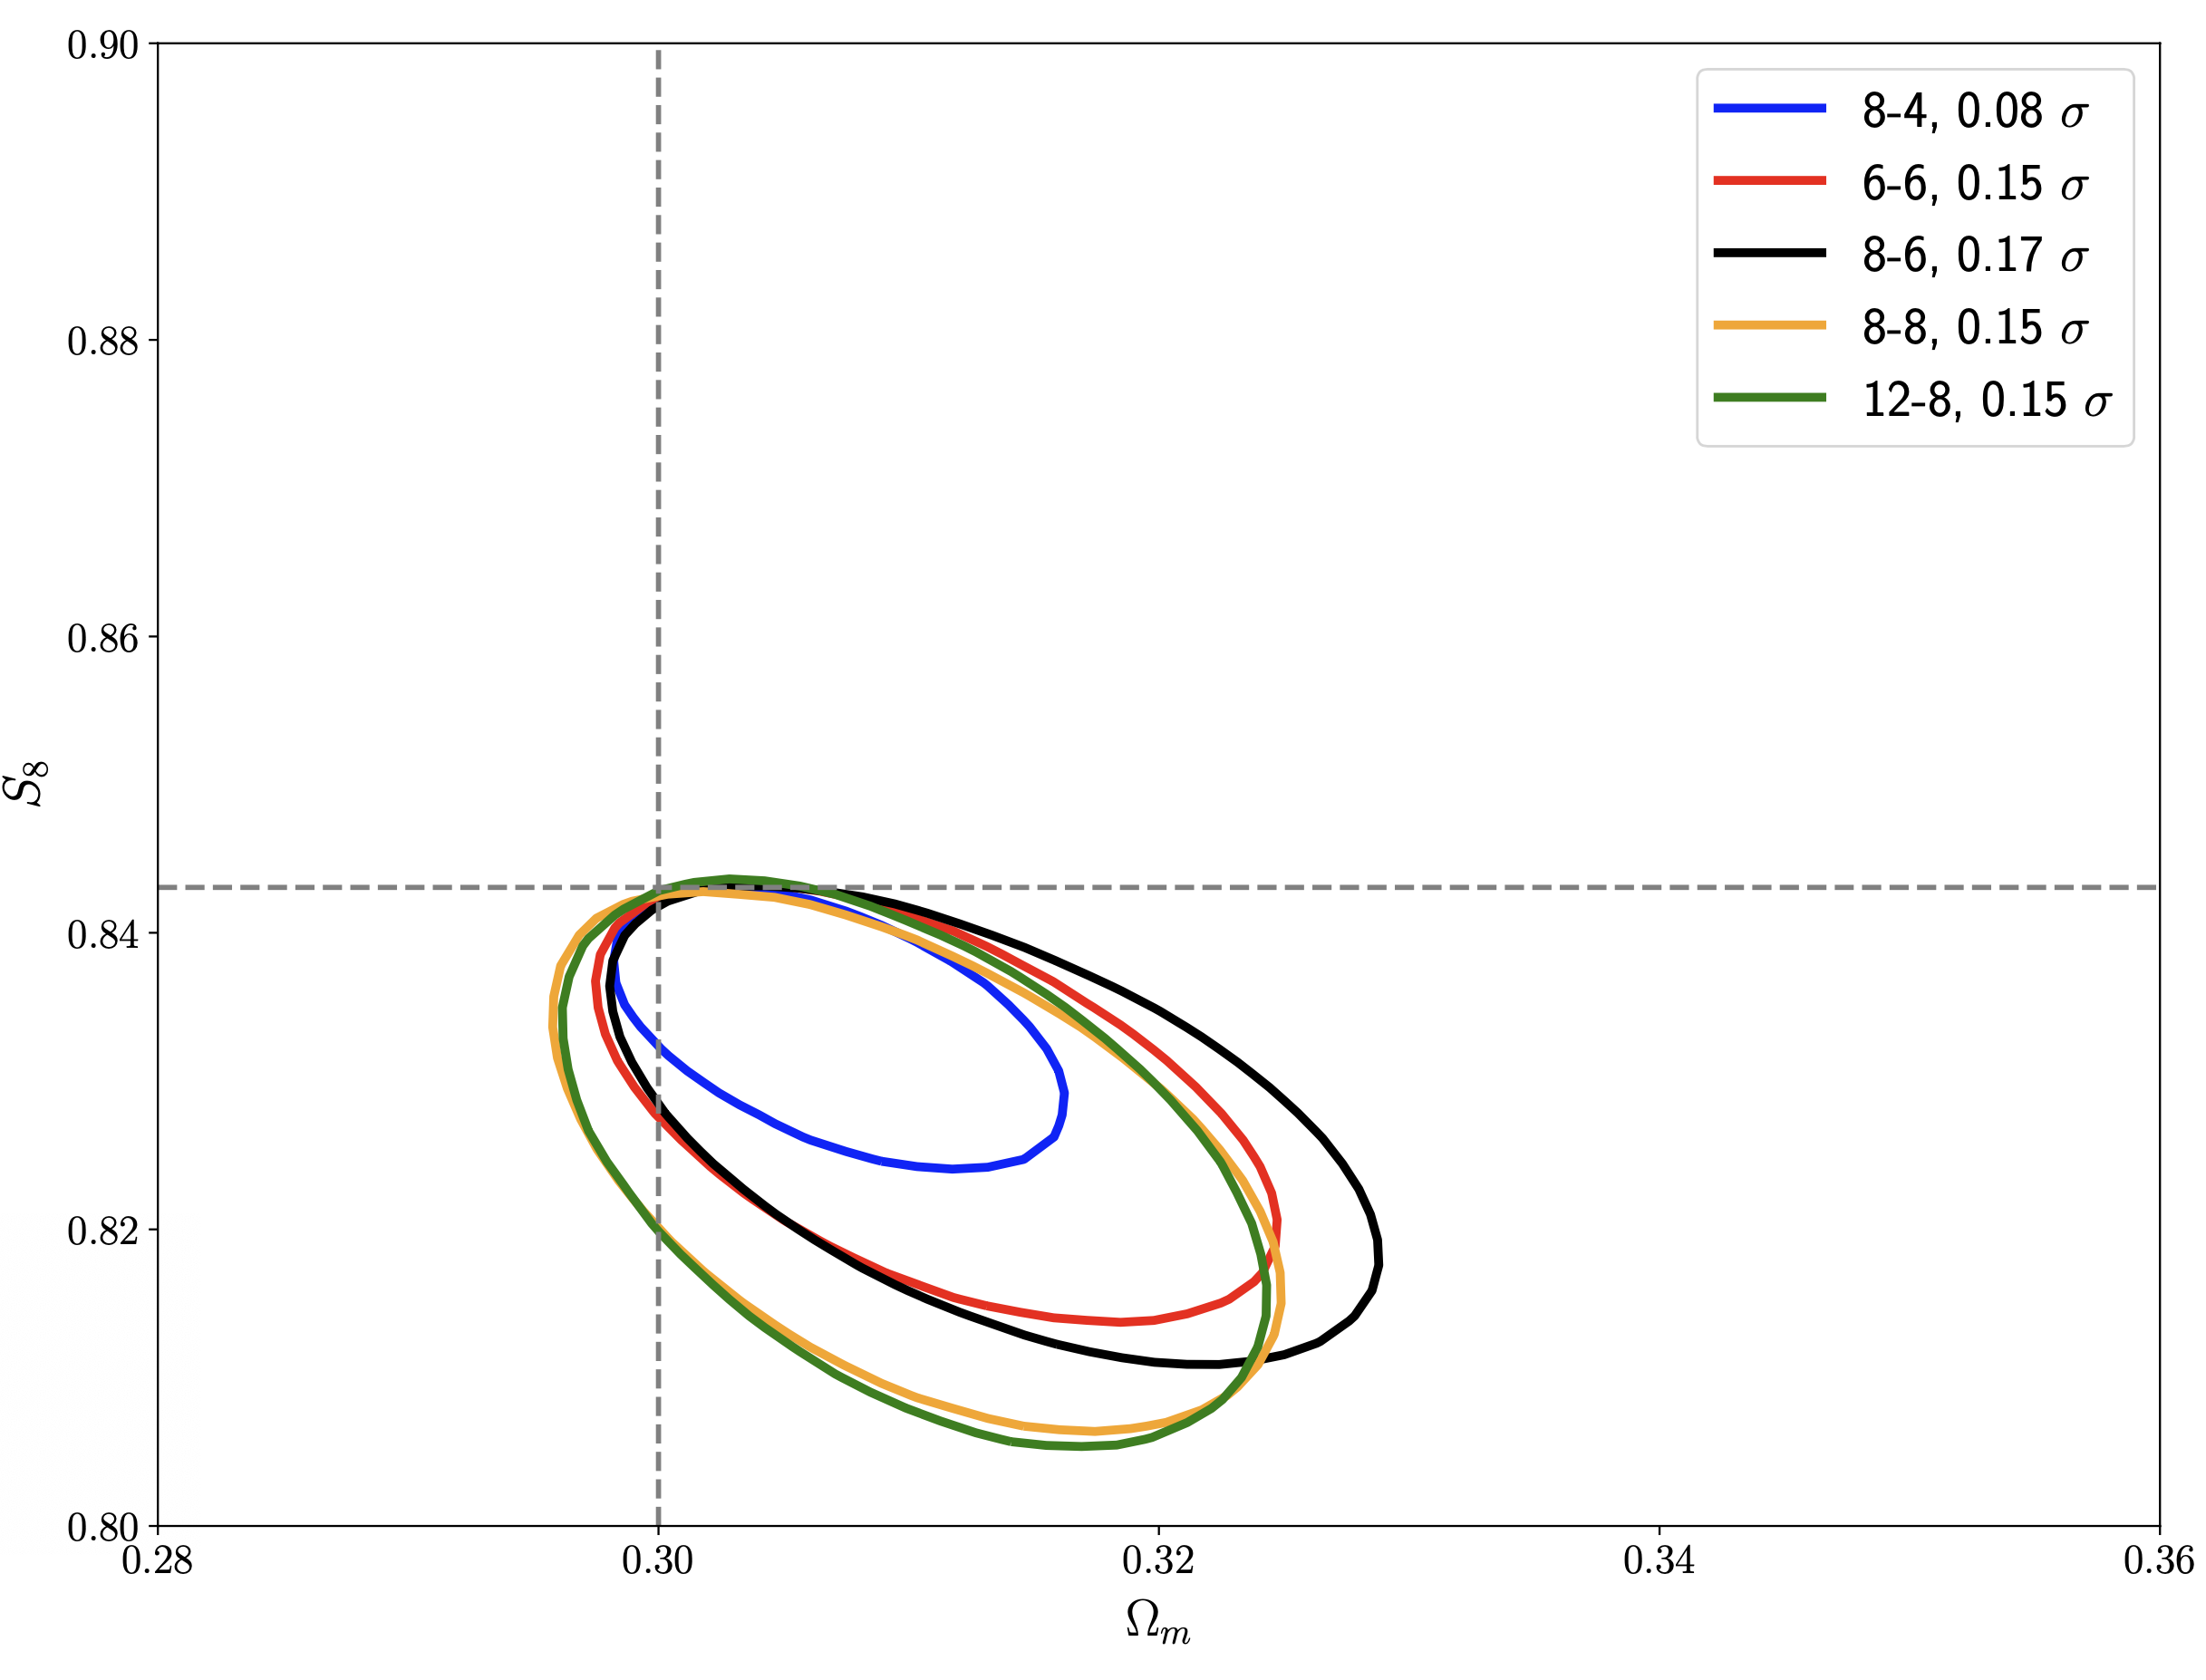
\includegraphics[width=0.5\textwidth,draft]{figs/temp.png}
\caption[]{Comparison of n(z)'s of sources and lenses in the data and in the \buzzard/\mice simulation. }
\label{fig:nz_comp}
\end{figure}

The datavectors, along with the best-fit theory models, for both the simulations and DES data are shown in the Appendix~\ref{app:2x2pt_measure}. 

\section{Validation of parameter inference}

\subsection{Models, scale cuts, priors and external datasets}
In this section we describe the models, scale cuts, priors and external datasets used.

\subsubsection{DES 2 $\times$ 2pt models + priors}
\label{sec:2x2pt_models}
We test three different galaxy bias model and prior choice combinations:
\begin{enumerate}
    \item Model A: Linear bias: As described in \S~\ref{sec:2pt}, the simplest model galaxy bias model is the  linear bias model. For each lens tomographic bin, the average bias of galaxies is given by a single free parameter $b_1$. We use a wide uninformative and uniform prior on the parameter for each lens tomographic bin $j$, given by $0.5 < b^{j}_1 < 4$. 
    \item Model B: 1-loop PT with the uninformative prior $-5<b_2<5$ for each lens bin, and $b_s, b_{3nl}$ fixed to the co-evolution Lagrangian values. This is a more complete model motivated by 1-loop effective field theory. In general, this model has five free bias parameters for each lens tomographic bin. However, from our tests on DES simulations (see 3D bias), we find that fixing two of them to their co-evolution value and the higher-derivative $k^2$ term to zero is sufficient to model our datavector down to 4Mpc/$h$. We use this  approximation to fit $w(\theta)$ and $\gamma_t$. However, we find that using a uniform prior on the linear and non-linear bias parameters leads to large projection effects. We choose to sample the parameters $b^{j}_1 \sigma_8$ and $b^{j}_2 \sigma^2_8$ which helps in removing much of the projection effect. We use wide uninformative uniform priors on these parameters for each tomographic bin $j$ given by : $0.67 < b^{j}_1 \sigma_8 < 3.0$ and $-4.2 < b^{j}_2 \sigma^2_8 < 4.2$. 
    \item Model C: Free all bias parameters, with the uninformative priors $-5<b_2<5, -5<b_s<5, -5<b_{3nl}<5$ ($b_k$?).
\end{enumerate}

\subsubsection{Scale cuts}
Motivated by the 3D bias modelling paper, we choose 2 or 3 sets of scale cuts.

From the tests on 3D correlation functions at fixed cosmology in simulations, we find that the linear bias approximation (Model A) is a good description above 8Mpc/$h$ while the two parameter non-linear bias model (Model B) can describe the correlations above 4Mpc/$h$.

\subsection{Cosmological models, external datasets and priors}
We test the following cosmological model and prior combinations
\begin{enumerate}
    \item Flat \lcdm\ with uninformative priors: We free five cosmological parameters $\Omega_m$, $\Omega_b$, $n_s$, $h_0$ and $A_s$. (\SP{or will we update all the results with free neutrinos?})
    % \item Flat \lcdm\ with informative priors on some combination of $\Omega_m$, $H_0$ and $n_s$ TBD.
    \item Flat \wcdm : In addition to above mentioned five parameters, we also free $w_0$.
    \item Flat \wcdm\ with Planck.
\end{enumerate}



\subsection{Simulated Likelihood tests}\label{sec:simlike_analysis}


We perform simulated likelihood tests to reveal which of our analysis choice combinations (i.e. scale cuts + bias model + priors + external dataset + cosmological model) return unbiased cosmological parameters.

\subsubsection{Scale cuts for linear bias model}
Motivated by the 3D bias modelling paper, we choose 2 or 3 sets of scale cuts.

% Due to an increase in the parameter space (as we sample over cosmological parameters as well as other systematics parameters described in \S~\ref{sec:full_pk_th}) as well as decrease in signal to noise (compared to noiseless 3D correlation functions), 

Our baseline case assumes linear galaxy bias and no baryon impact on the matter-matter auto power spectrum. The linear bias values that we use for the five lens bins are $b_1 = 1.7, 1.7, 1.7, 2.0$ and  $2.0$  respectively. We compare the cosmology constraints from the baseline datavector with a simulated datavector having contamination from higher order non-linearities. The contaminated datavector receives contribution from non-linear bias and baryonic physics. For non-linear bias we use  Model B (see \S~\ref{sec:2x2pt_models}) with non-zero $b_2, b_s$ and $b_{\rm 3nl}$ terms. The value of $b_2$ used in the contaminated datavector is given by the interpolated $b_1-b_2$ relation extracted from 3D tests in \mice simulations (see Fig.8 of 3D draft) for each tomographic bin. We also fix the bias parameters $b_s$ and $b_{\rm 3nl}$ to their co-evolution values. To capture the impact of baryons on the matter-matter power spectra, we use the feedback model of OWLS-AGN.

We define our criteria to identify  scale cuts in the 2D plane of the most constrained cosmological parameters. For $\Lambda$CDM cosmology, we use $\Omega_m - S_8$ while for $w$CDM cosmology we use $\Omega_m-S_8$, $\Omega_m-w_0$ and $S_8-w_0$. Our criteria for scale cuts is defined as the minimum scales which results in distance of the peak of 2D marginalized contours when analyzing the baseline datavector from the peak of contours when analyzing the contaminated datavector be less than 0.3$\sigma$. We find that for our linear bias model, the angular cuts corresponding to (8,6) Mpc/$h$ for $w(\theta)$ and $\gamma_t$ pass the above mentioned criteria. The resulting contours and the distances between the peak of the marginalized baseline contours, the peak of the marginalized contaminated contours and the input truth value for cosmological parameters is shown in Fig.~\ref{fig:sim_lin}. 

\SP{\begin{itemize}
    \item \textbf{\textit{Figure}} Linear bias recovering unbiased cosmology (for $\Lambda$CDM) at scale cut (X,Y) Mpc/$h$. Show contours also for one scale cut smaller and one scale cut bigger than this. 
    \item \textbf{\textit{Figure}} Linear bias $w$CDM: Show results for $w$CDM with and without Planck
    \item \textbf{\textit{Figure}} Non-linear bias $\Lambda$CDM: Show the results for non-linear bias LCDM recovering true cosmology when the input bs and b3nl are not given by co-evolution relation but model uses those relations.
\end{itemize}
}




\begin{figure*}
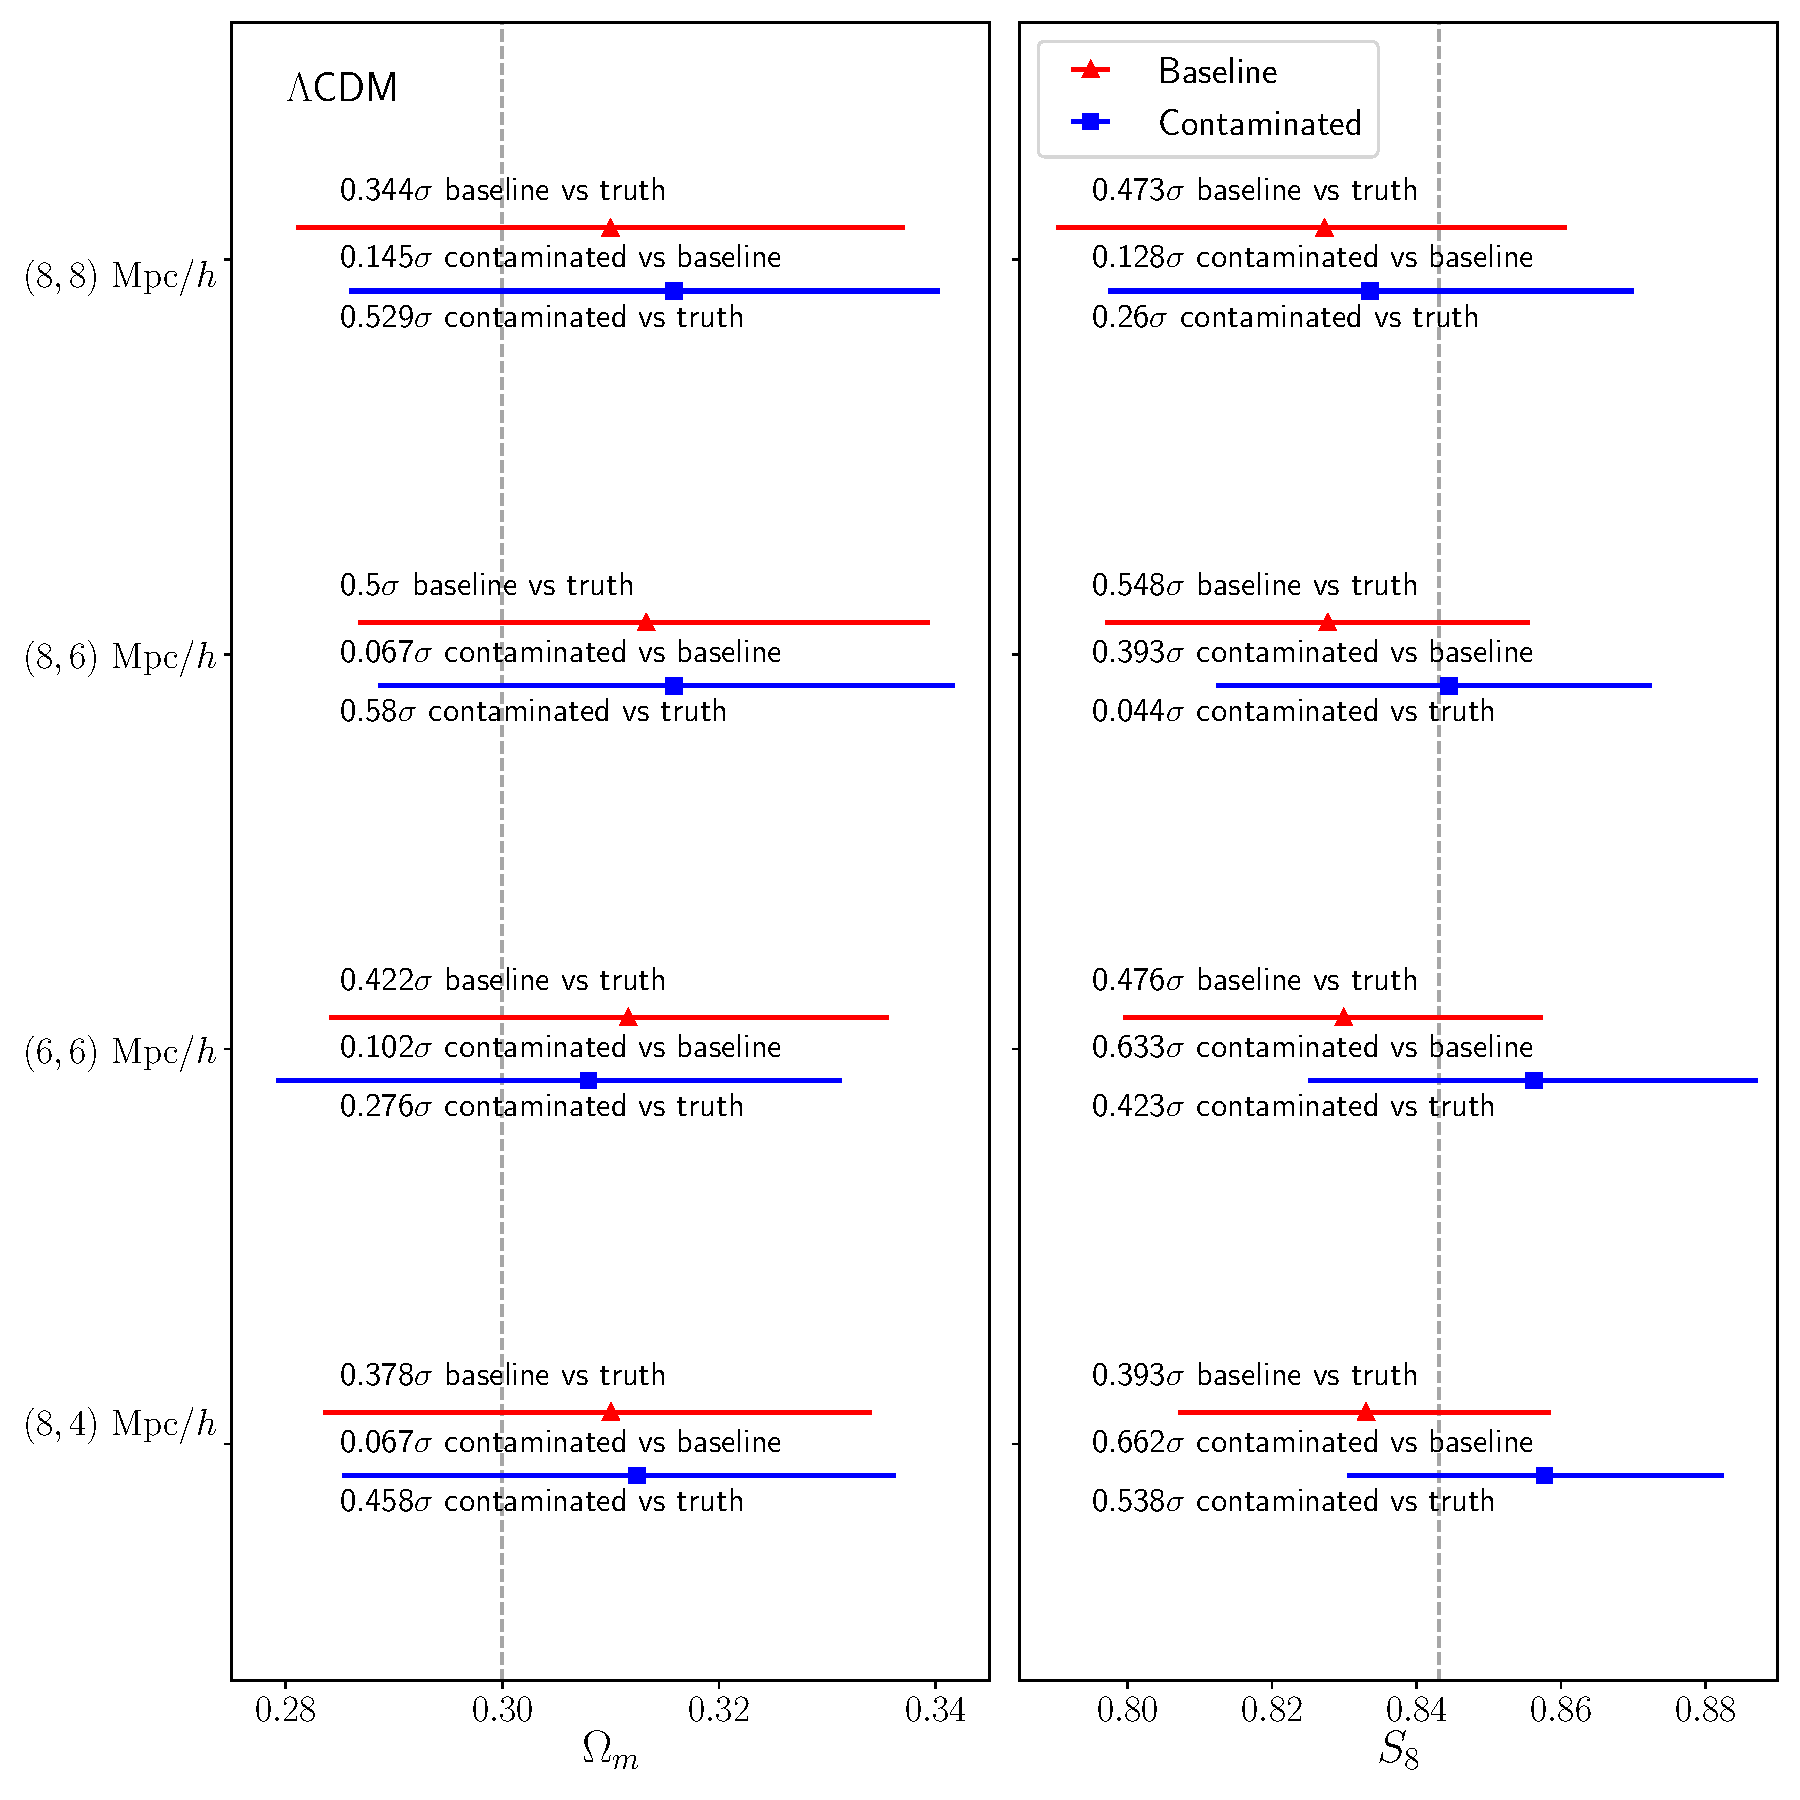
\includegraphics[width=\columnwidth]{figs/2x2pt_1dmarg_lcdm_paper.pdf}
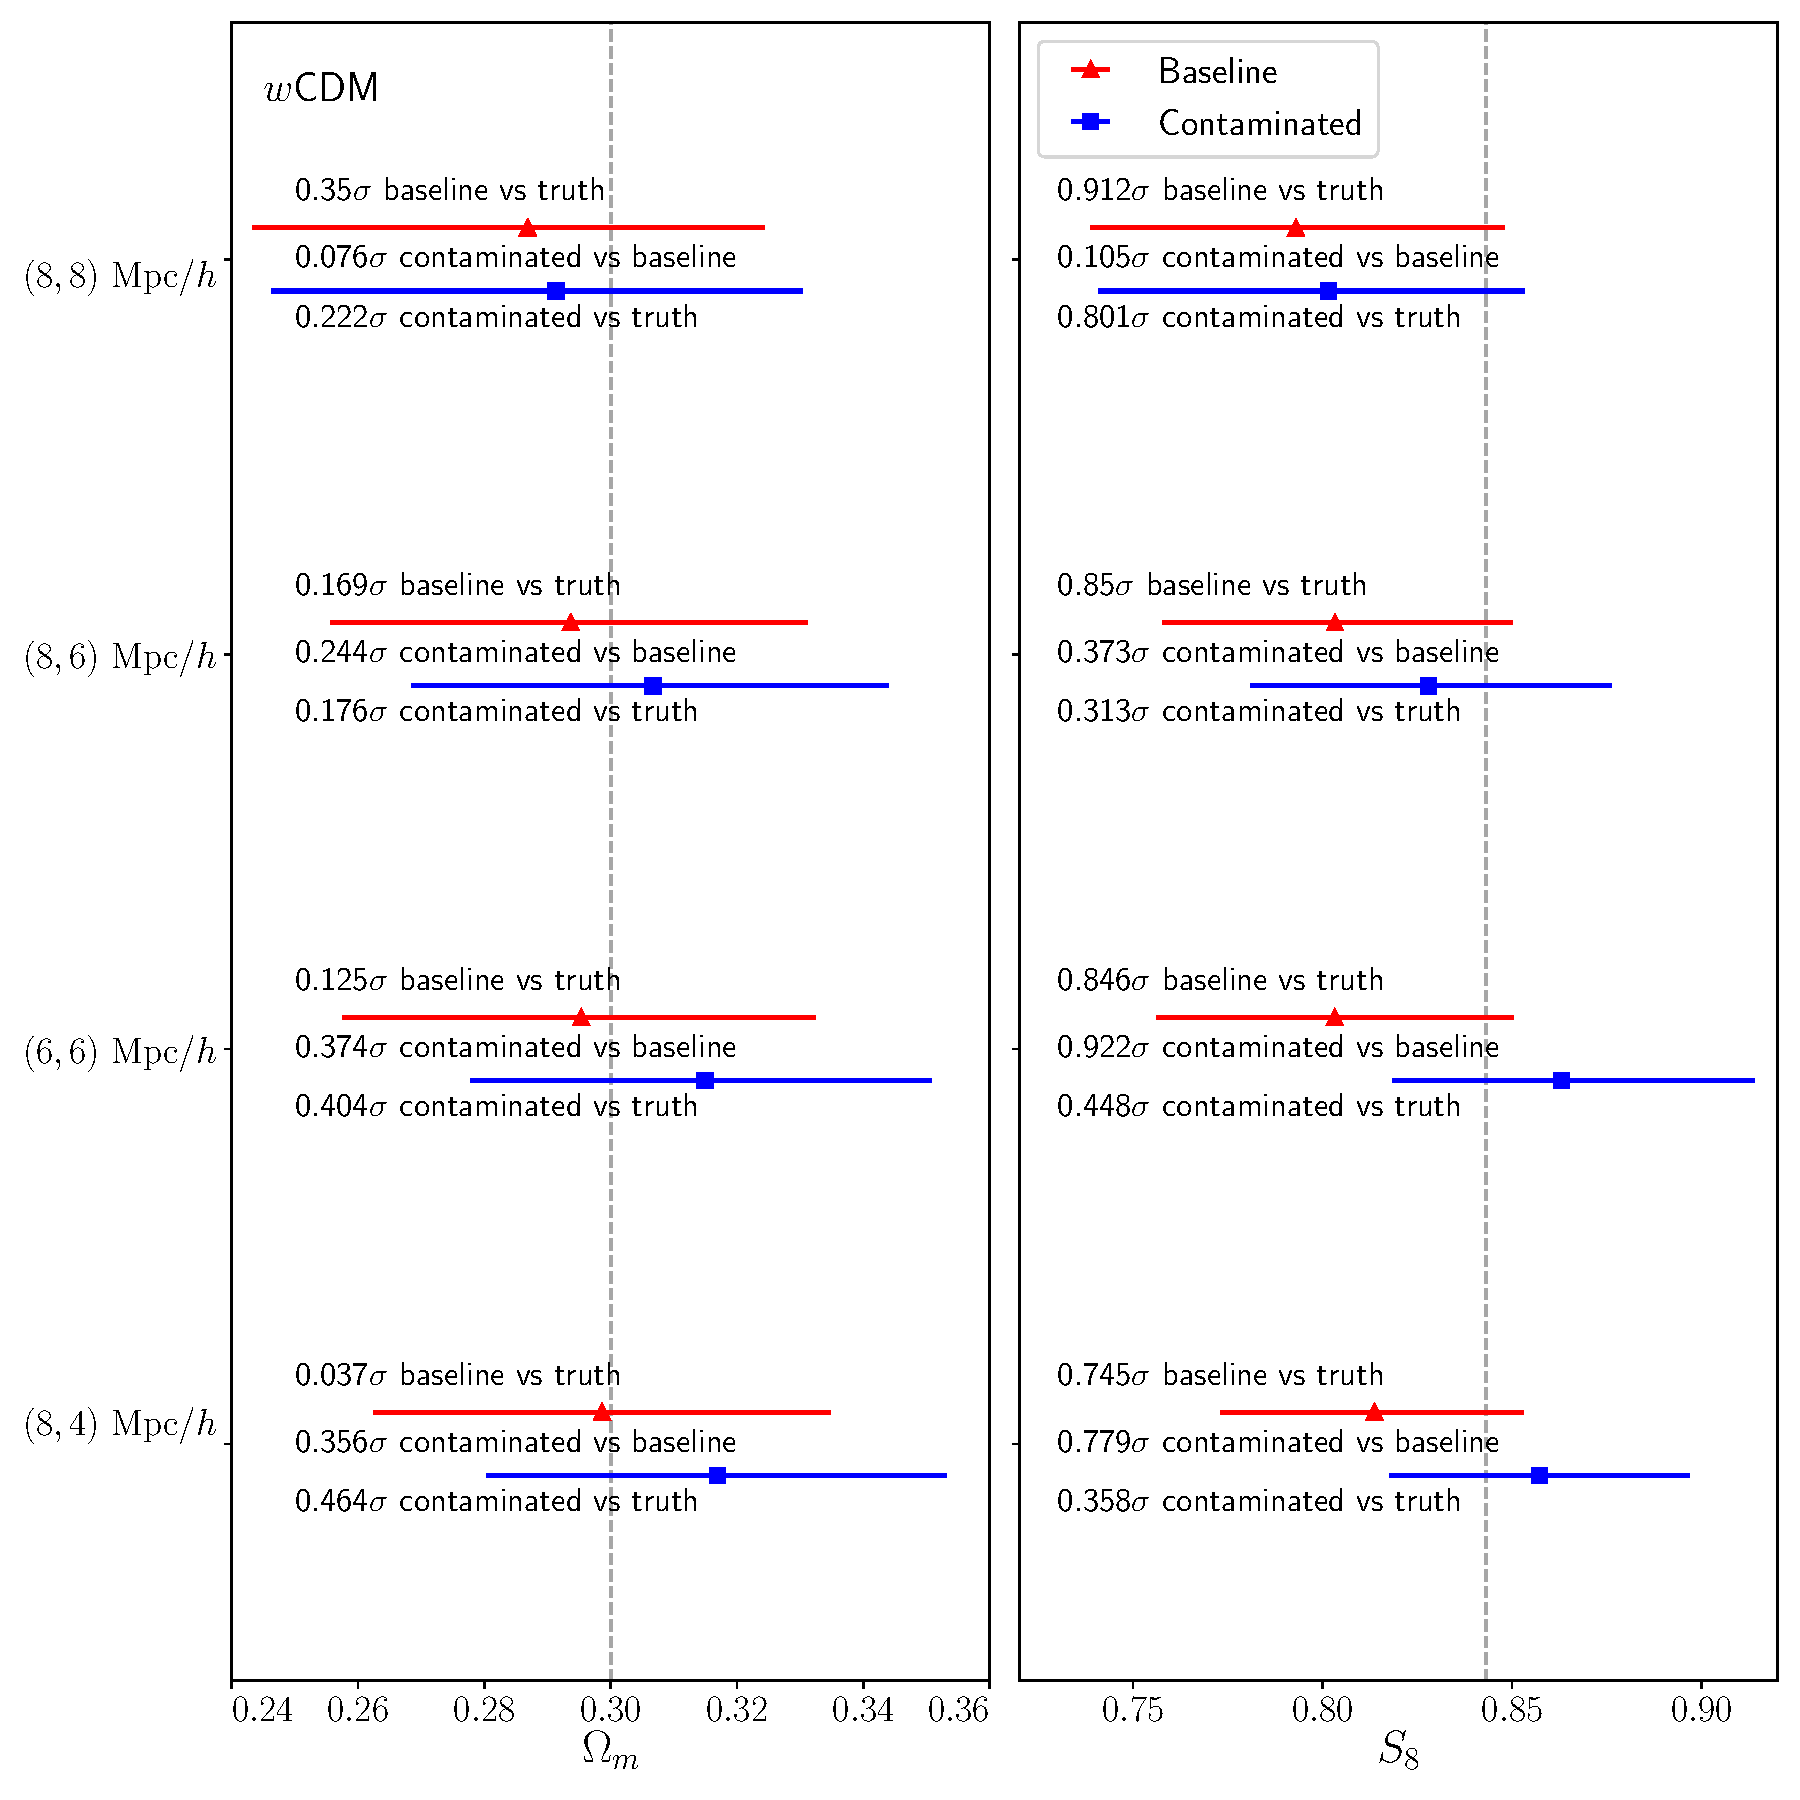
\includegraphics[width=\columnwidth]{figs/2x2pt_1dmarg_wcdm_paper.pdf}
\caption[]{Simulated likelihood analysis when analyzing a datavector contaminated with non-linear bias + baryons and analyzed with linear bias + halofit as the model. The two panels on the left show \lcdm while the panels on the right show \wcdm. For each scale cut for (\wtheta,\gammat) as indicated on the y-axis labels, we compare the recovered cosmological  constraints for the contaminated datavector and baseline datavector (with zero contamination). There are residual biases in both $\Omega_m$ and $S_8$ even in baseline case (due to projection effects, see \S\ref{sec:simlike_analysis} and Appendix \ref{app:projection_effects}), the difference between constraints from the baseline and contaminated datavector gets larger as we go down in scale cuts along y-axis. We use the criterion of difference between contaminated and baseline being greater than X$\sigma$, to choose our fiducial scale cuts for the linear bias model as (X,Y)Mpc/$h$.    }
\label{fig:sim_lin}
\end{figure*}


\begin{figure}
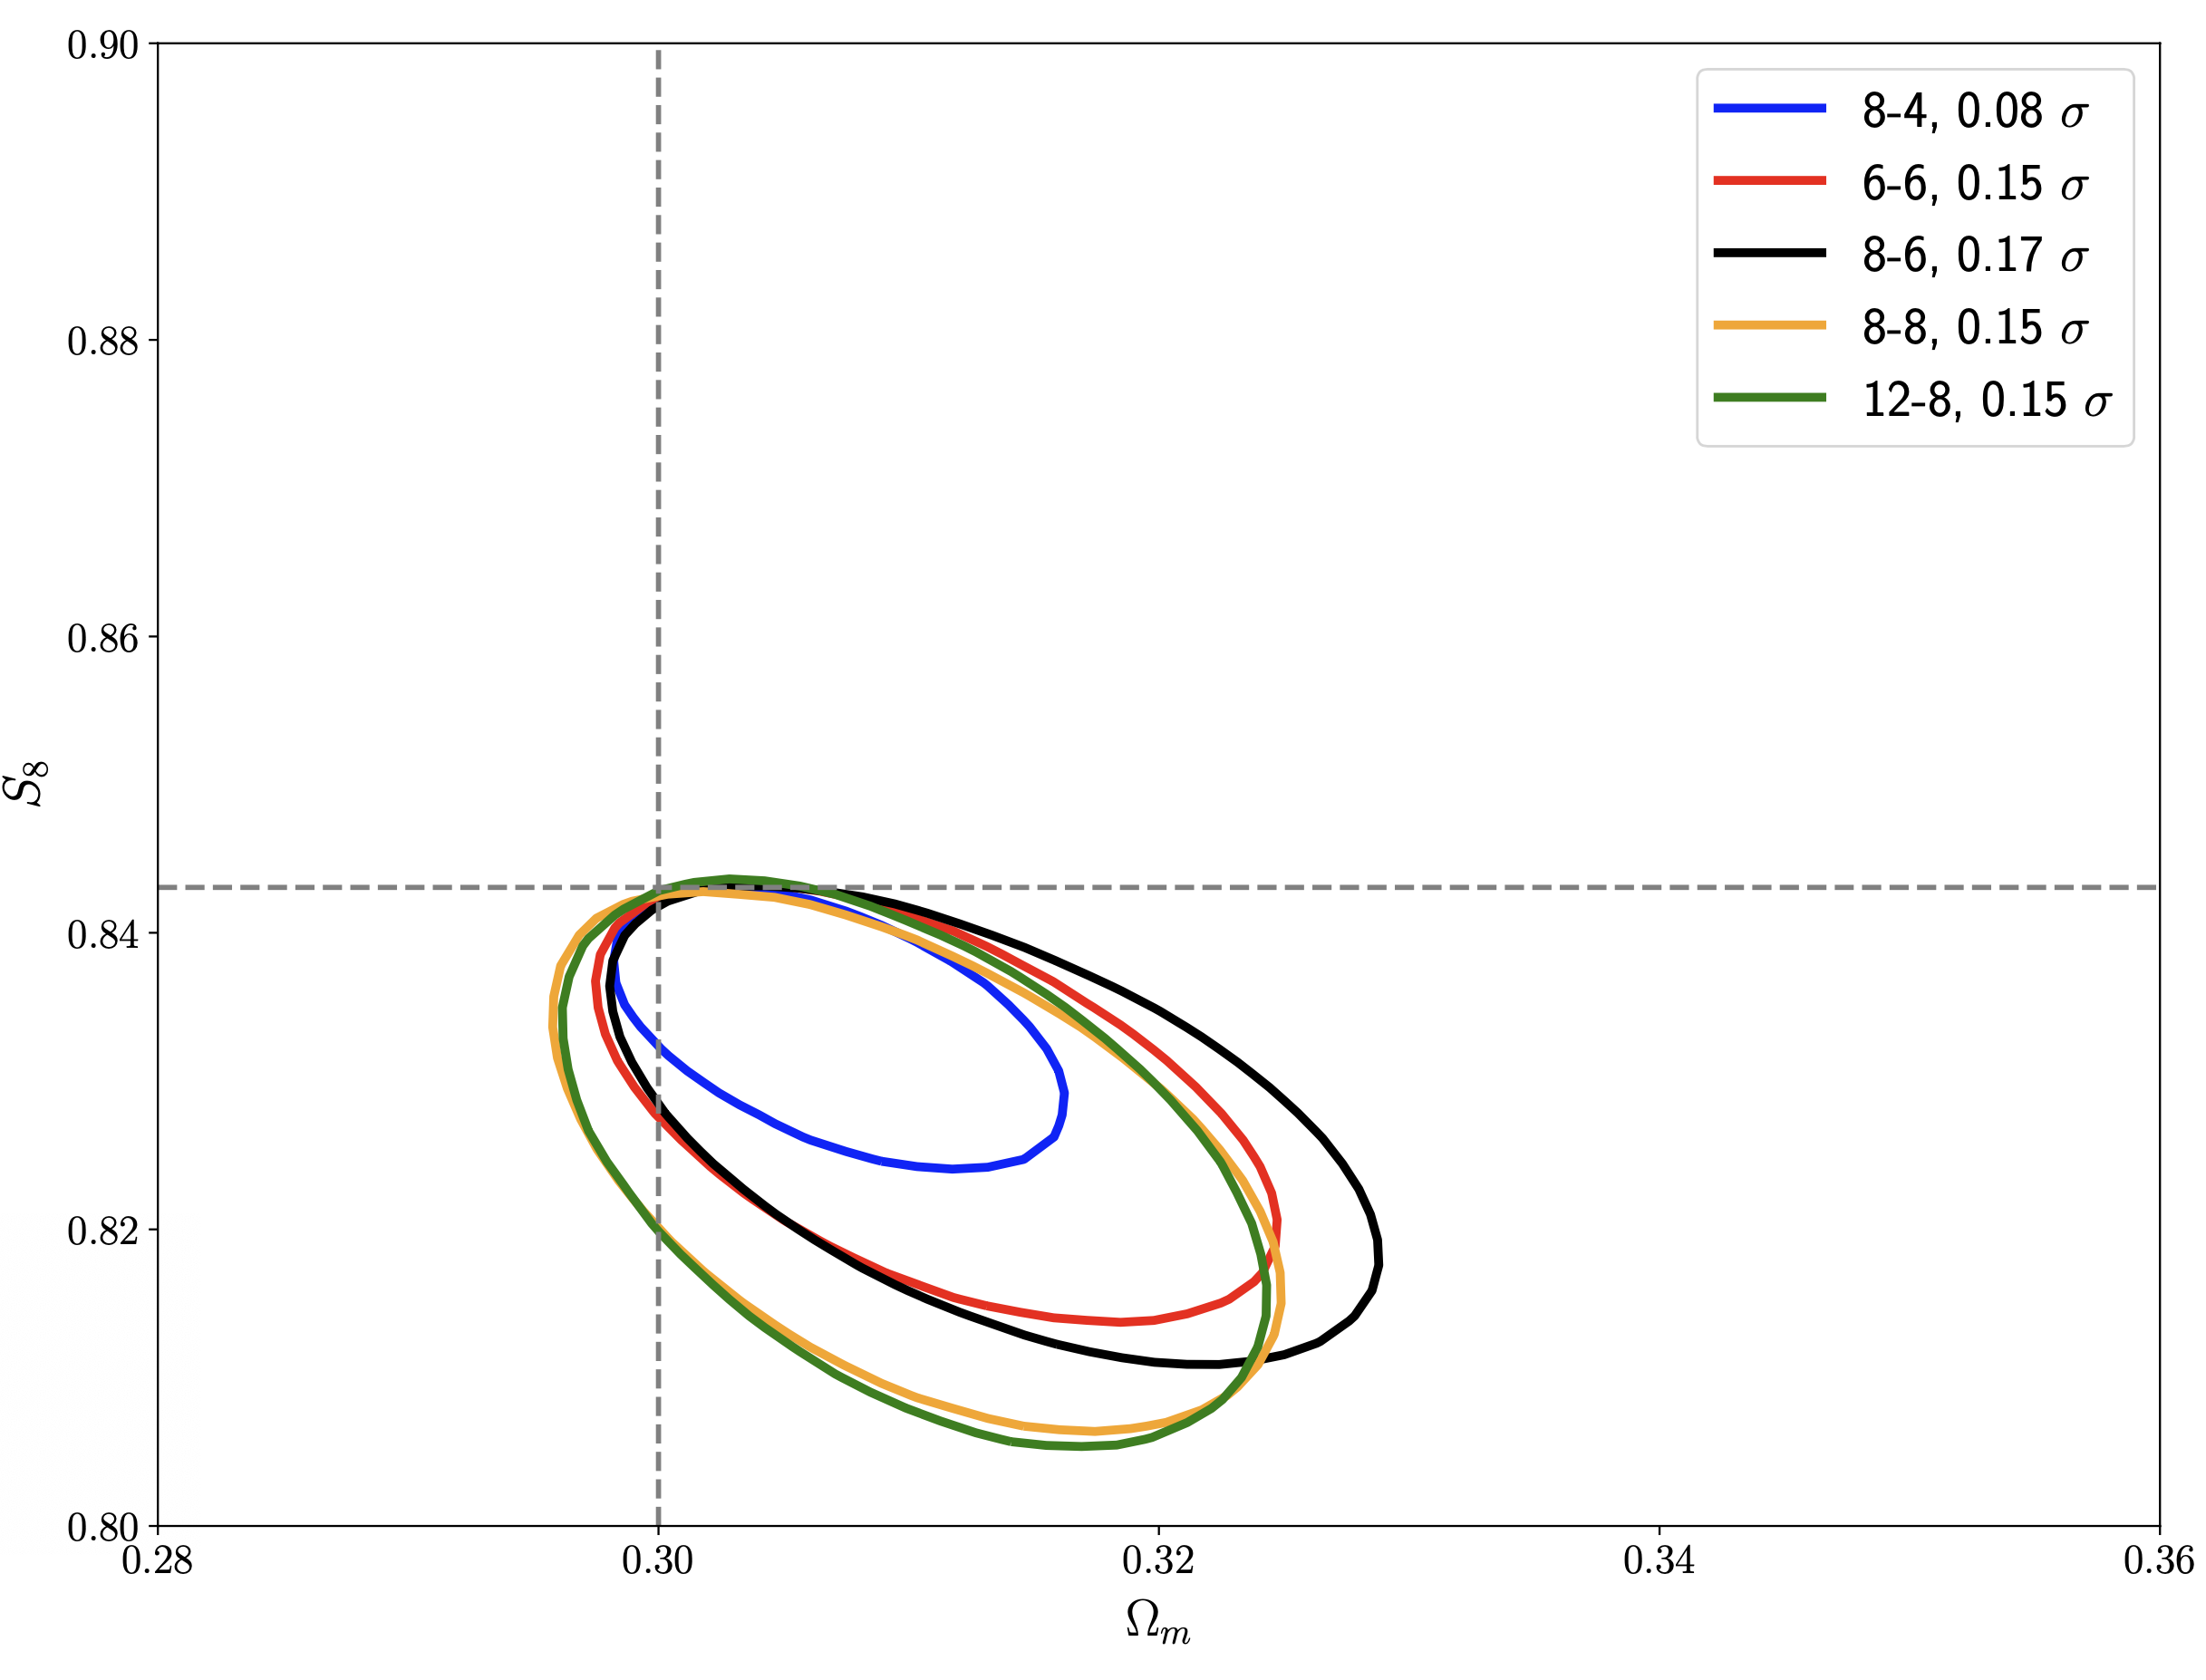
\includegraphics[width=0.5\textwidth,draft]{figs/temp.png}
\caption[]{Comparison of 1D or 2D $\Omega_m-S_8$ contours when analyzing with fiducial non-linear bias model ($b_s$ and $b_{\rm 3nl}$ fixed to co-evolution value) a datavector with $b_s$ and $b_{\rm 3nl}$ shifted by 1$\sigma$ (as given by 3D tests). This will validate our fiducial non-linear bias model from a simulated likelihood method. }
\label{fig:nlbias_comp}
\end{figure}

\subsection{Results on Buzzard simulations}

For  analysis choice combinations that pass the simulated likelihood tests, we validate on the suite of Y3 \buzzard simulations. We will select analysis choice combinations that return unbiased cosmological parameters to run on the data. 

\subsubsection{DES-only \lcdm}

\begin{figure*}
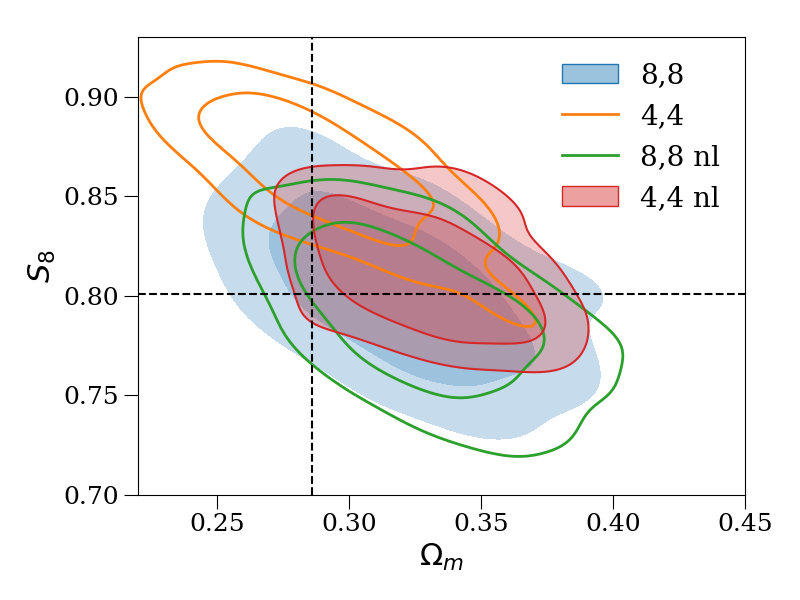
\includegraphics[width=\columnwidth]{figs/buzzard_lcdm_om-s8.png}
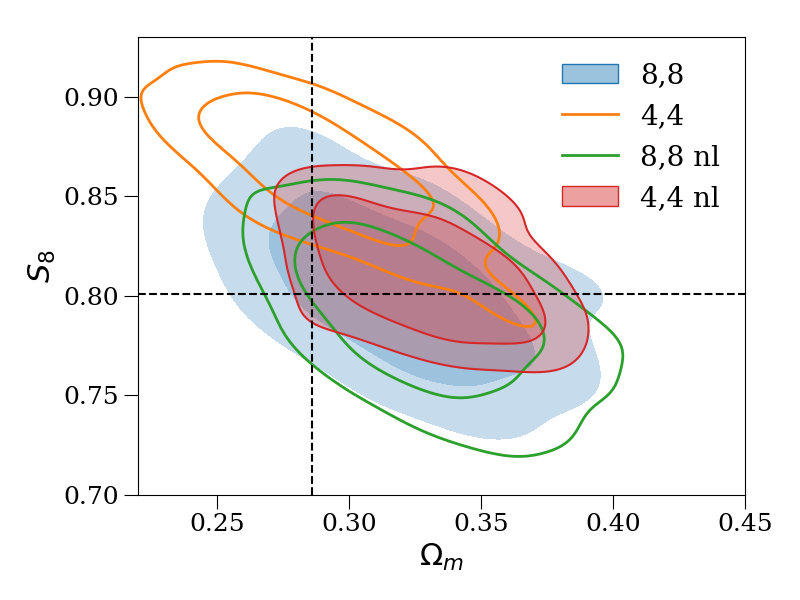
\includegraphics[width=\columnwidth]{figs/buzzard_lcdm_om-s8.png}
\caption[]{\lcdm\ Buzzard constraints, we show the constraints on $\Omega_m$ and $S_8$ from the mean (over all N realizations) Buzzard 2x2pt measurements, with cosmological parameter priors set I (i.e. wide, ~uninformative priors) in the left panel, and set II in the right panel. We show constraints with two sets of scale cuts: 4,4 and 8,6. In each panel we show constraints for linear and non-linear galaxy bias models. Comment on which of the options give unbiased cosmology. Use this figure to set the scale cuts for non-linear bias model as well.  }
\label{fig:bcc_des_lcdm}
\end{figure*}

In \fig{fig:bcc_des_lcdm} we show the constraints on $\Omega_m$ and $S_8$ from the mean (over all N realizations) Buzzard 2x2pt measurements, with cosmological parameter priors set I (i.e. wide, ~uninformative priors) in the top panels, and set II in the bottom panels. We show constraints with two sets of scale cuts: 4,4 (left panels) and 8,8 (right panels). In each panel we show constraints for all galaxy bias models (i)-(iv). Comment on which of the options give unbiased cosmology. 

\SP{
\begin{itemize}
    \item \textbf{\textit{Figure}} Linear bias: Based on results on simulated likelihood test, show the cosmology constraints using linear bias model on N-buzzard simulations. 
    \item \textbf{\textit{Figure}} Non-linear bias : Show the $\Omega_m - S_8$ constraints on few scale cuts motivated by the 3D tests. 
\end{itemize}
}


\subsubsection{\wcdm\ with Planck}

\begin{figure*}
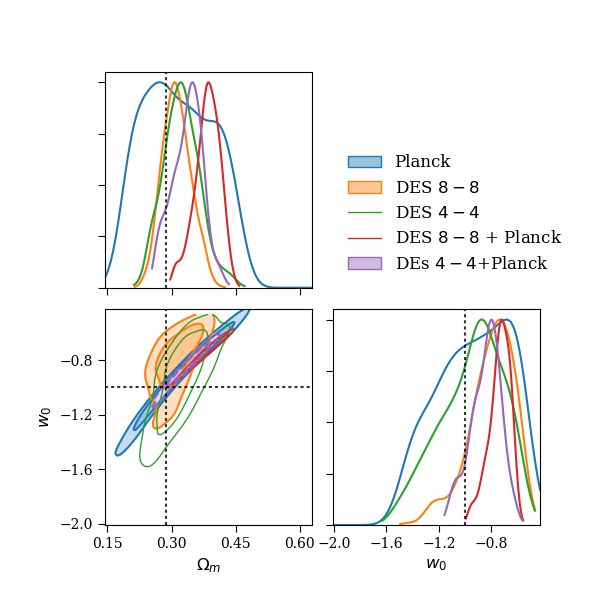
\includegraphics[width=\columnwidth]{figs/buzzard_wcdm_lin_om-w.png}
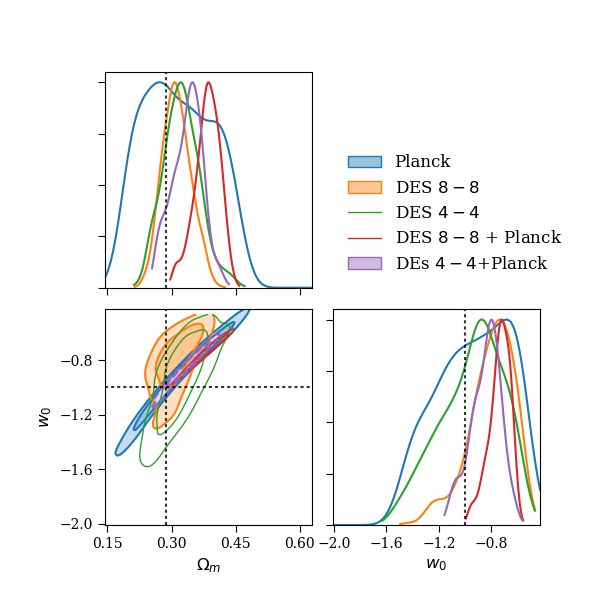
\includegraphics[width=\columnwidth]{figs/buzzard_wcdm_lin_om-w.png}
\caption[]{\wcdm\ Buzzard constraints, linear bias (left panel), non-linear bias (right-panel). Show the constraints with DES alone as well as when using with Planck.}
\label{fig:color_ims}
\end{figure*}

In \fig{fig:bcc_des_wcdm} we show the constraints on $\Omega_m$ and $w$ from the Buzzard 2x2pt measurements, and also simualted Planck CMB data (simulated at the Buzzard cosmology). We use only cosmological prior set I here (but now with free $w$). There'll be a plot for each choice bias model.

Also validate bias modelling choices at fixed cosmology?

\SP{
\begin{itemize}
    \item \textbf{\textit{Figure}} Linear bias: Based on results on simulated likelihood test, show the cosmology constraints using linear bias model on N-buzzard simulations. 
    \item \textbf{\textit{Figure}} Non-linear bias : Show the $\Omega_m - S_8$ constraints on few scale cuts motivated by the 3D tests. 
\end{itemize}
}



\section{Results}

\subsection{DES-only constraints}

Compare DES-only constraints for the three or four analysis variations. Hopefully they agree. Compare performance of different models and present fiducial constraint.

\SP{\begin{itemize}
    \item \textbf{\textit{Figure}} Compare the constraints from cosmic shear, 2x2pt and 3x2pt datavectors for the scale cuts defined for the 3x2pt $\Lambda$CDM analysis. Explain the loss of constraining power in 2x2pt compared to 3x2pt due to PM. Show for both linear bias and non-linear bias. 
\end{itemize}
}

\begin{figure}
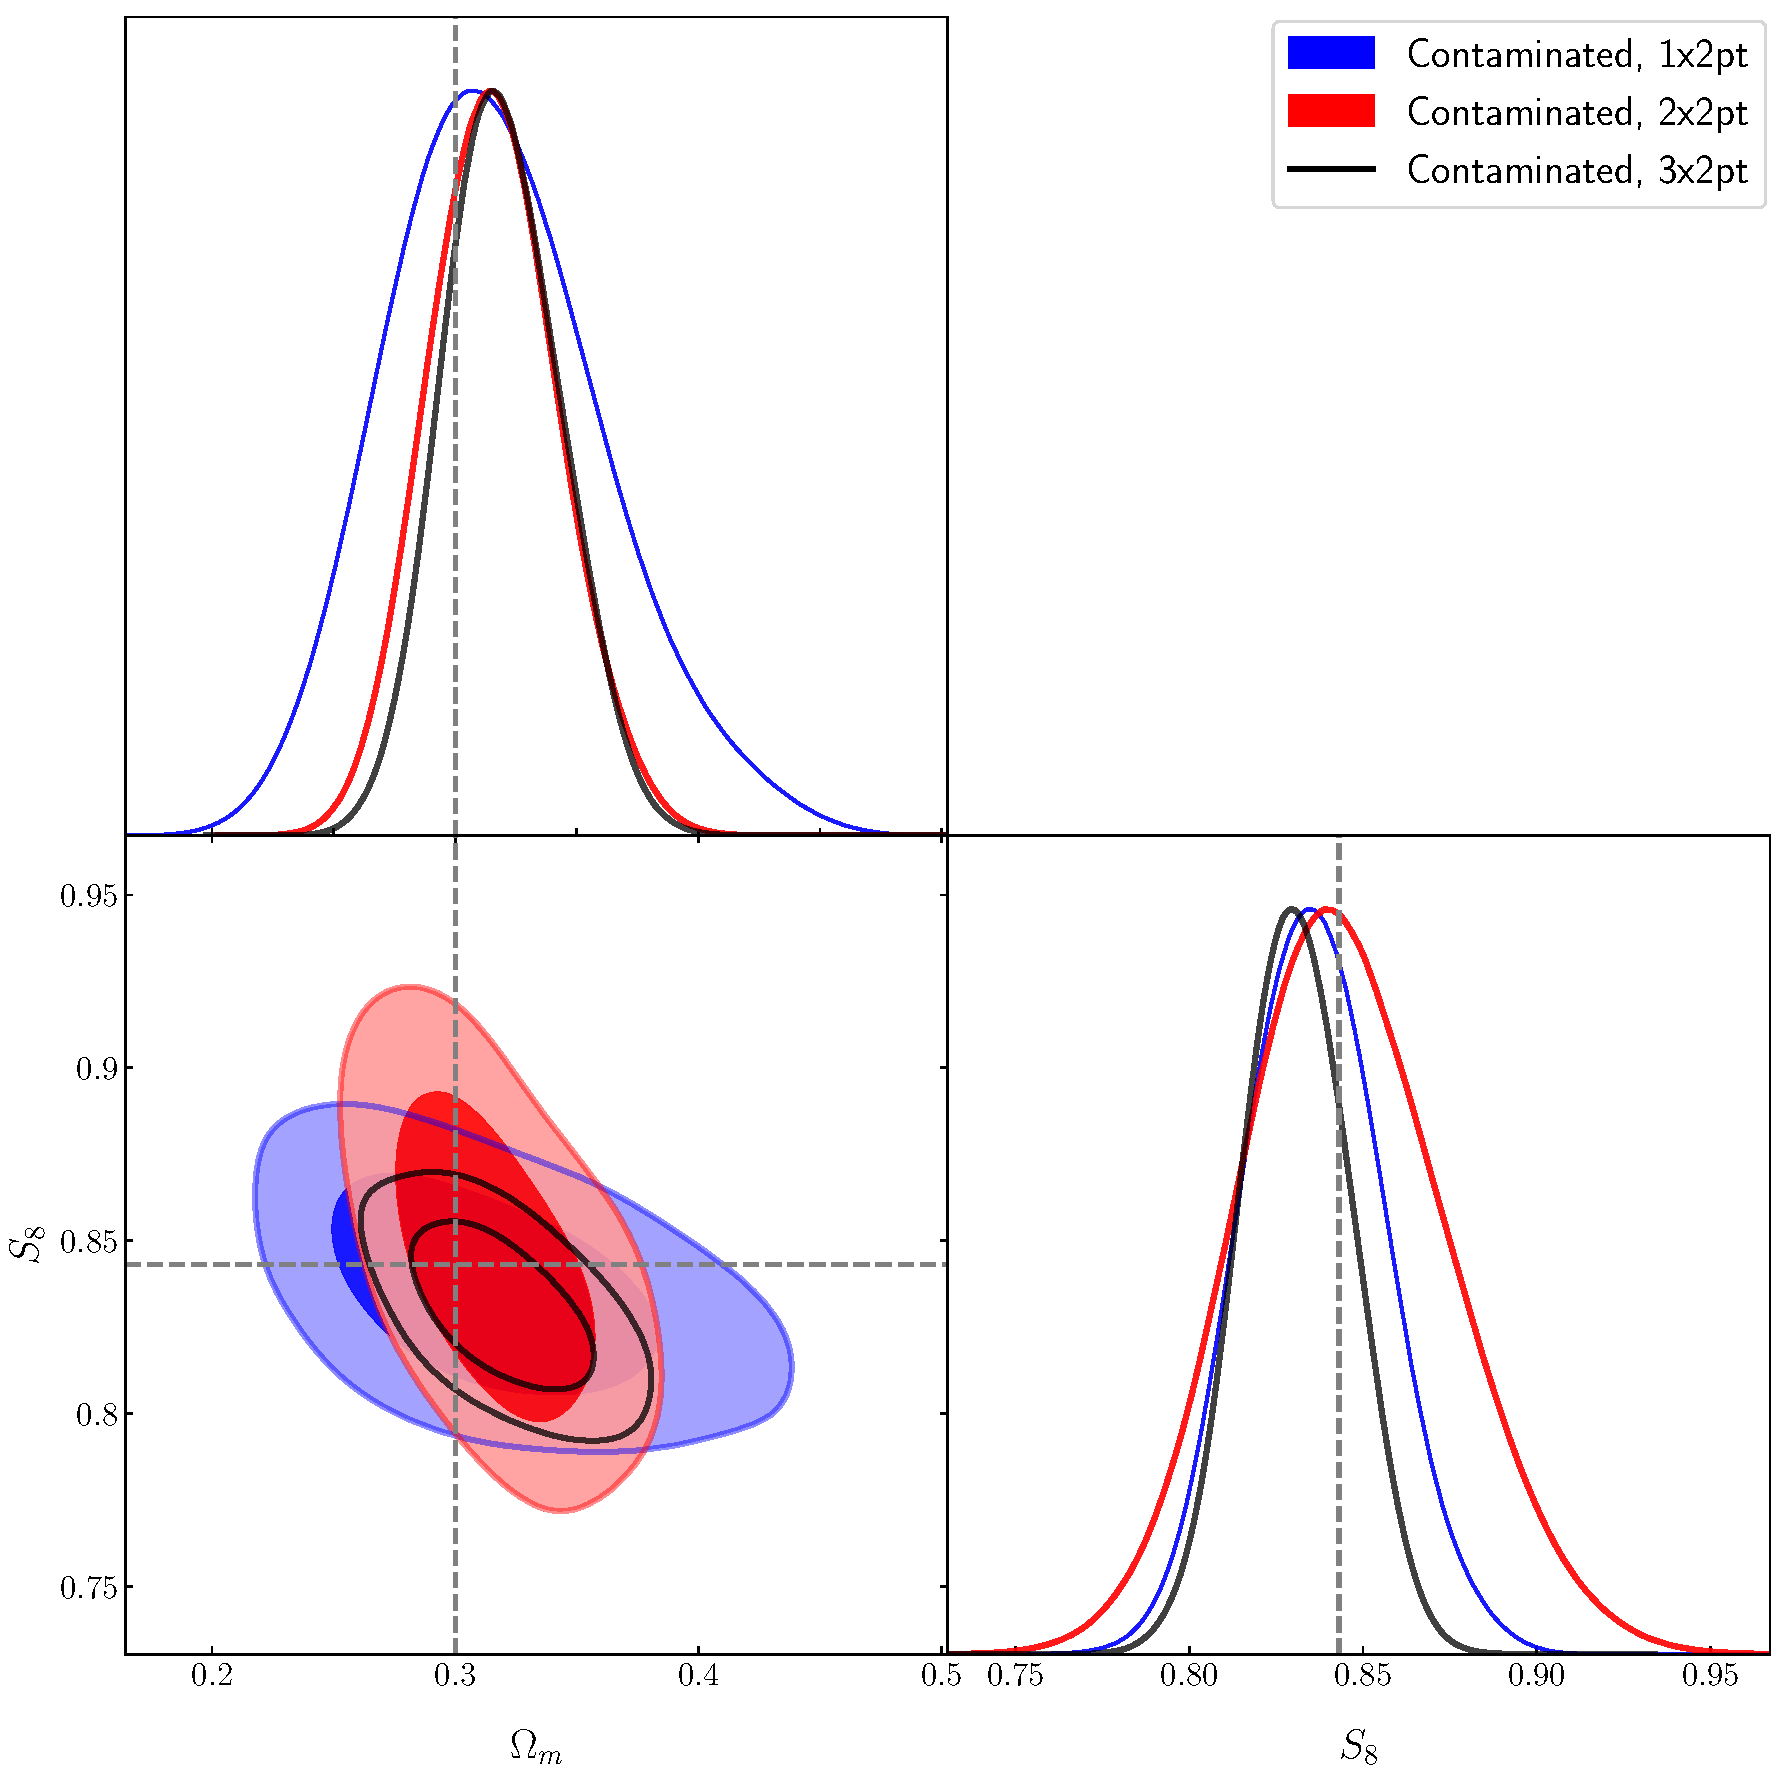
\includegraphics[width=\columnwidth]{figs/compare_all_cosmo_3x2pt_lcdm_contaminated.pdf}
\caption[]{Compare the constraints from cosmic shear,  2x2pt and 3x2pt  with linear bias + halofit model with the same scale cuts (preferably fiducial 3x2pt cuts) for $\Lambda$CDM. Show that cosmic shear and 2x2pt add complementary information with 2x2pt providing stronger constraints on $\Omega_m$ and cosmic shear providing constraints on $S_8$.}
\label{fig:des_comp}
\end{figure}

\begin{figure}
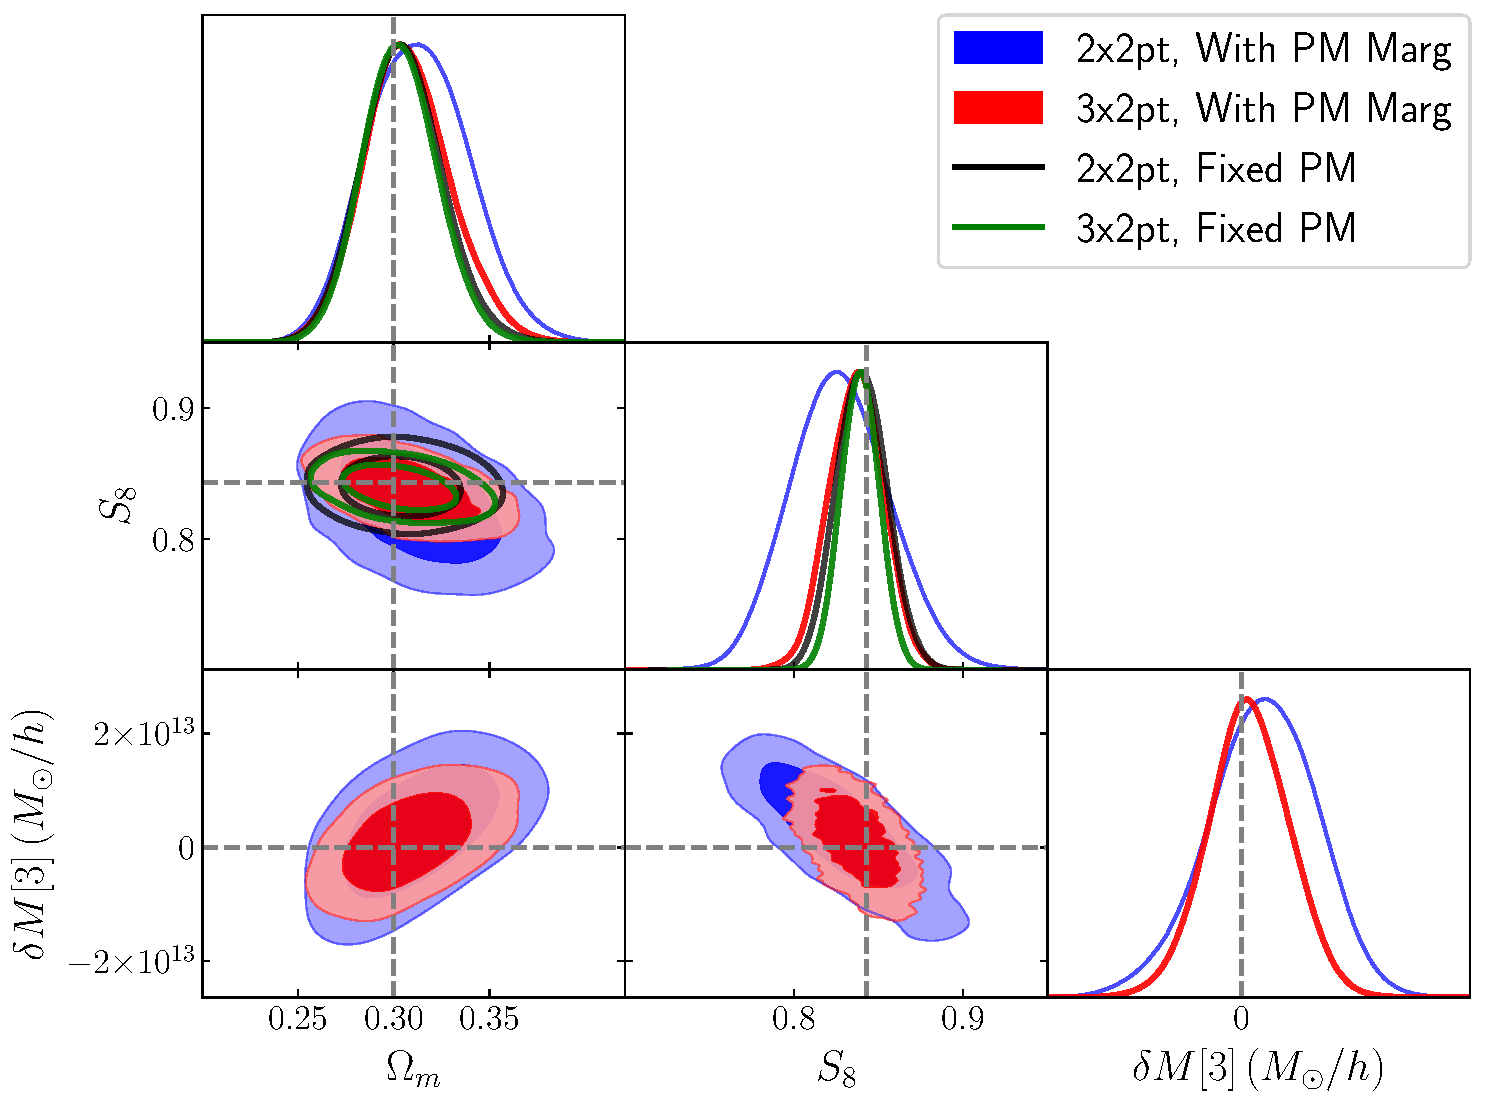
\includegraphics[width=\columnwidth]{figs/PM_constraints_2x2pt_3x2pt.pdf}
\caption[]{Effect of point mass marginalization on the constraining power of 2x2pt and 3x2pt. We see that the constraining power of 2x2pt degrades significantly with point mass marginalization, while for 3x2pt the change is minimal. Including the shear-shear correlation  breaks the degeneracy between point-mass (we show PM for third bin, $M_{\rm halo}[3]$) and $S_8$, leading to smaller sensitivity of cosmology constraints on point mass constraints. \SP{update the plot with non-zero PM in DV, to show the biases as well} }
\label{fig:pm_effect}
\end{figure}

\begin{figure}
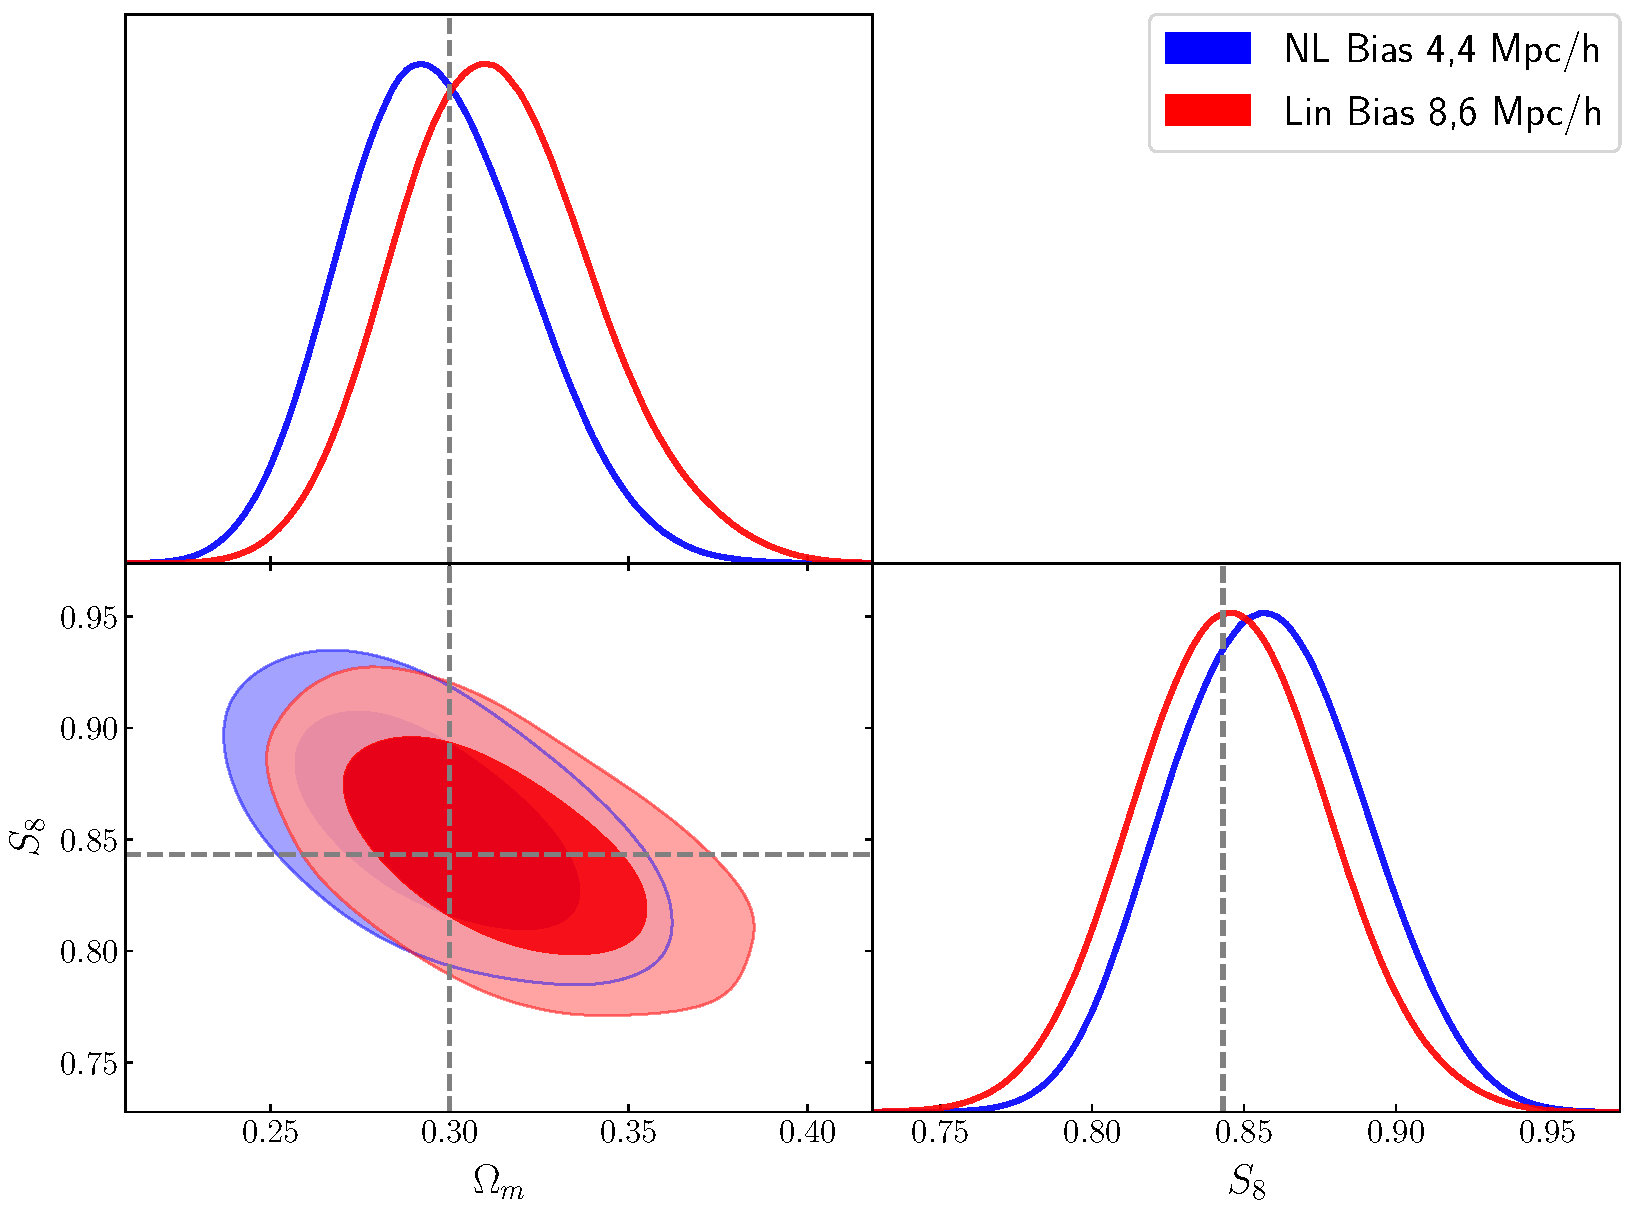
\includegraphics[width=\columnwidth]{figs/compare_cosmo_nl44_lin86.pdf}
\caption[]{Compare the 2x2pt $\Lambda$CDM constraints for both linear bias and non-linear bias at their respectively defined scale cuts. Show that using non-linear bias leads to more constraining power, especially in $\Omega_m$, with the ability to push down to smaller scales. }
\label{fig:des_comp}
\end{figure}



\subsection{Consistency with external datasets}

\subsection{DES+external constraints}

Cosmology and galaxy bias constraints from DES+external. Again compare performance of different analysis choices. Compare bias constraints with some theoretical expectations.

\begin{figure}
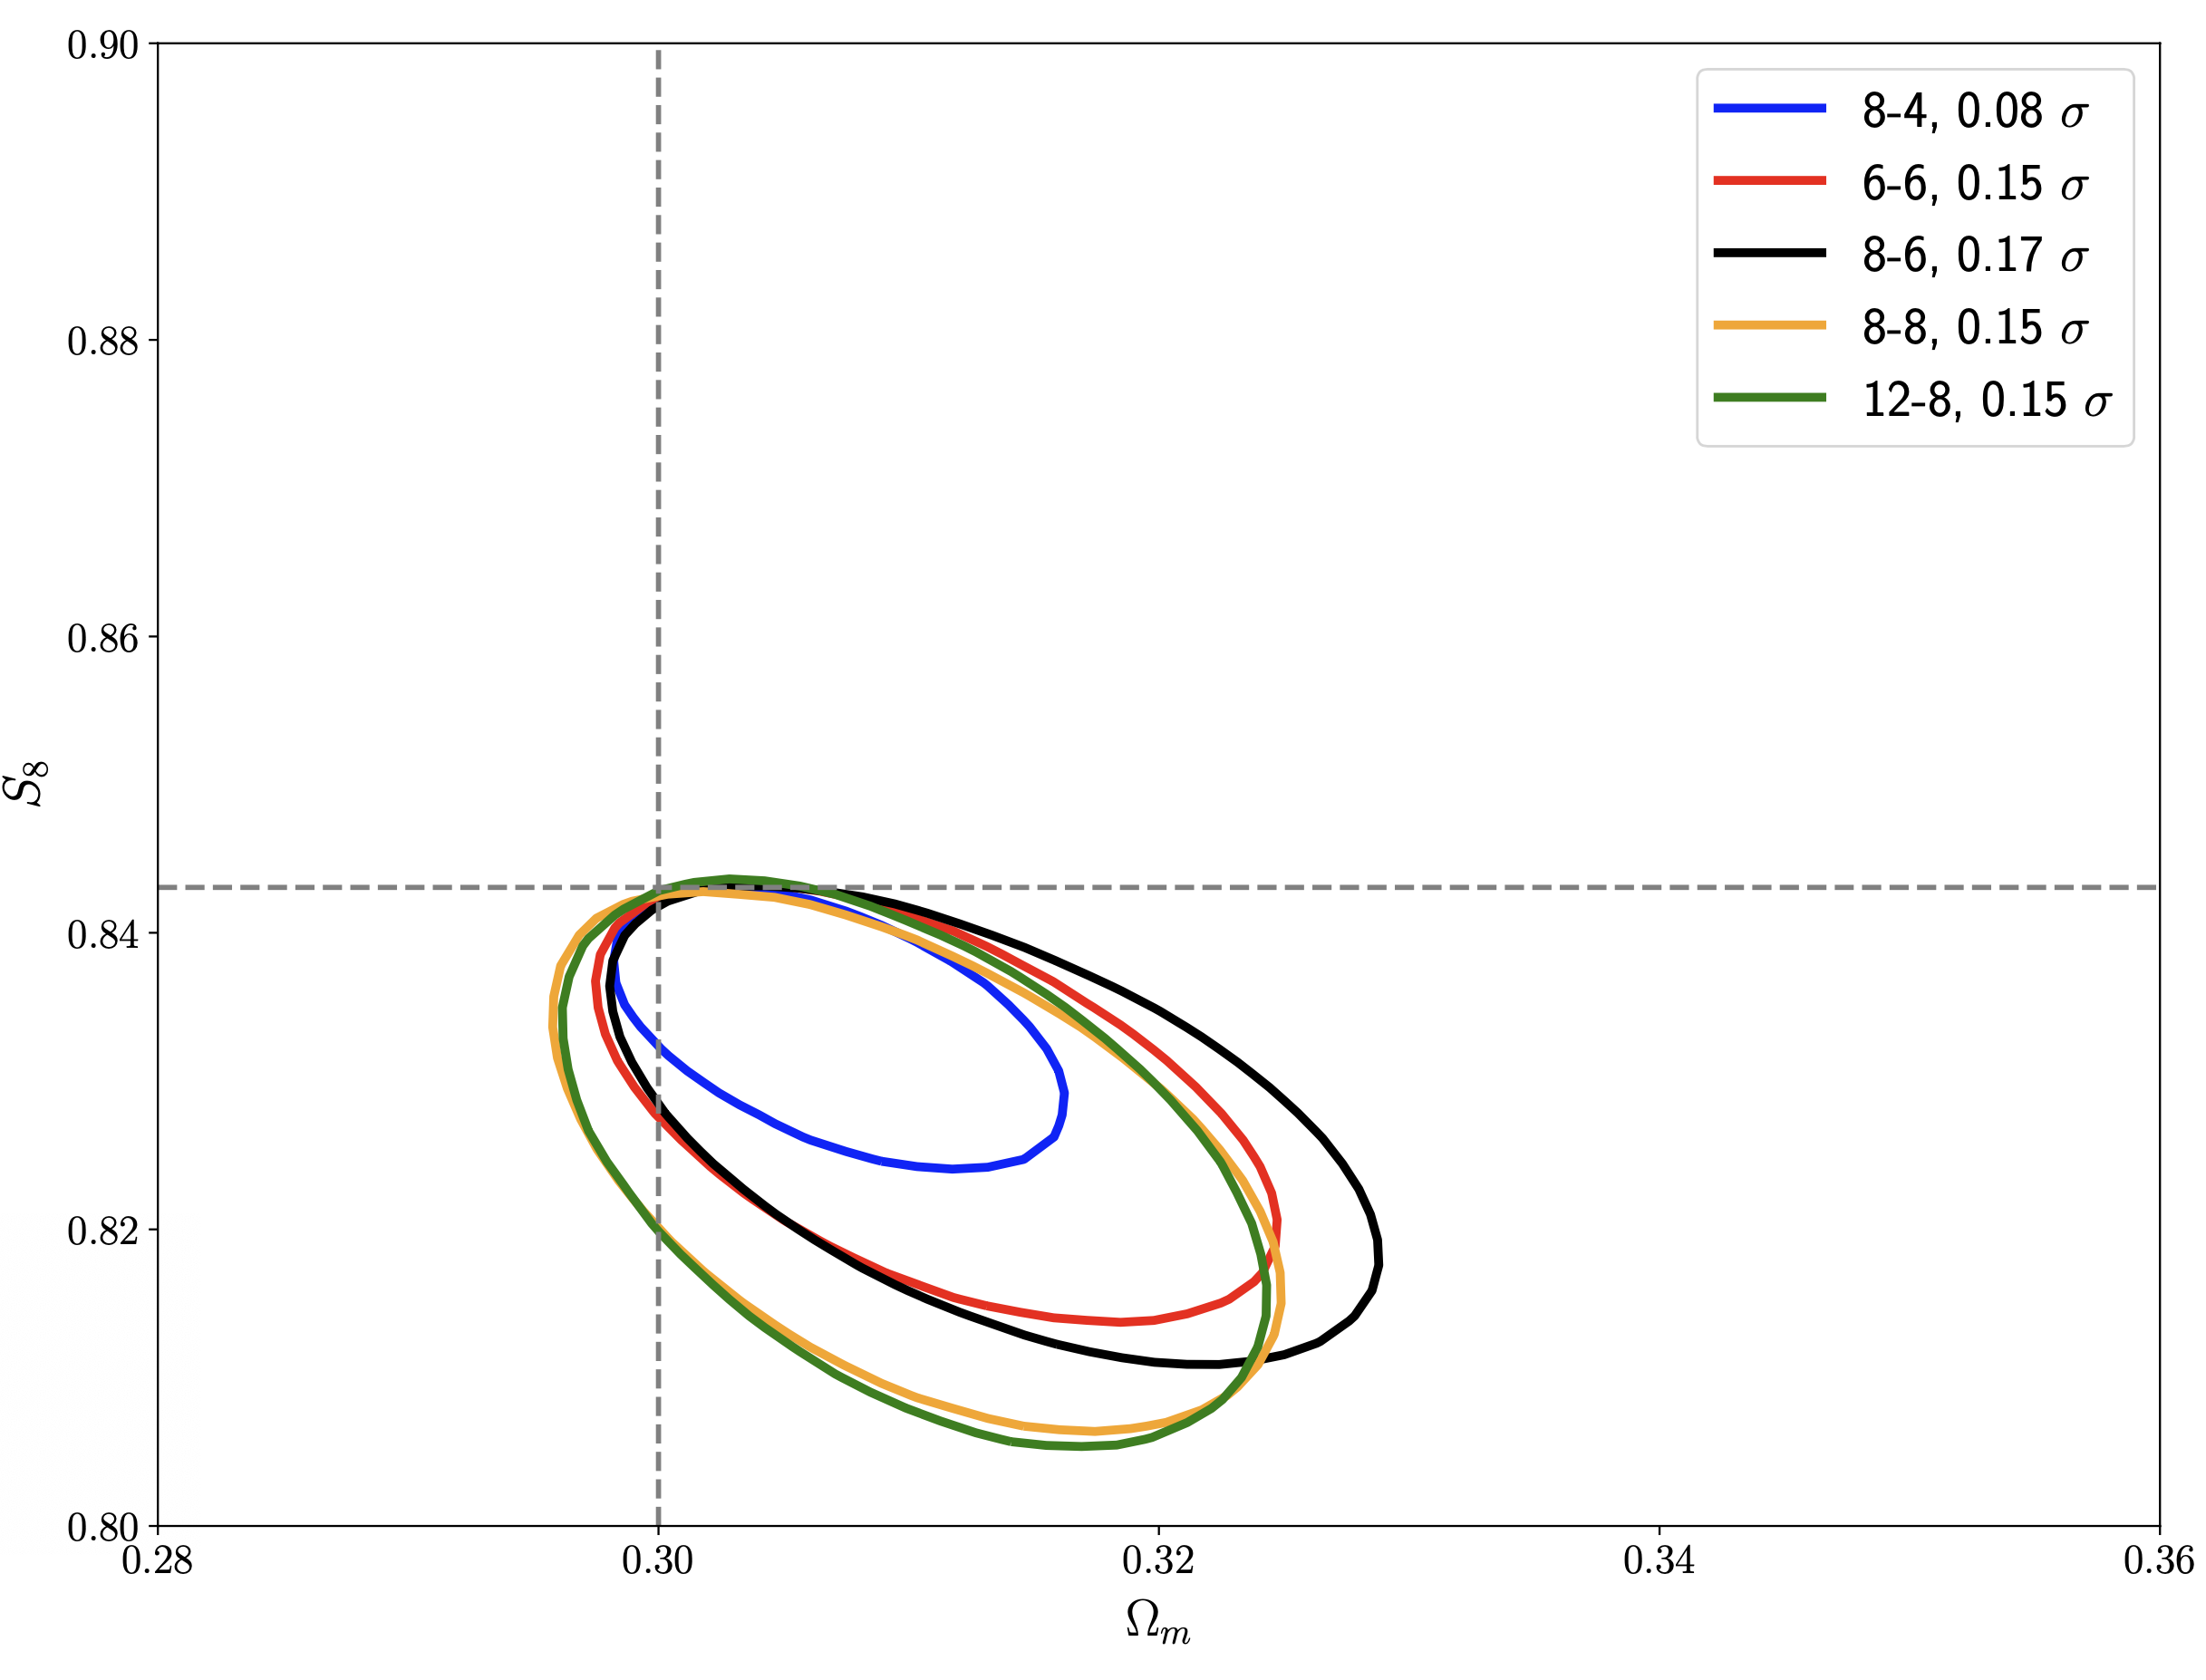
\includegraphics[width=\columnwidth,draft]{figs/temp.png}
\caption[]{Show the DES+external constraints for both \lcdm \ and \wcdm \ cosmologies. Show DES and external alone and their combination. Comment of their consistency and on their tension. }
\label{fig:bias_relation}
\end{figure}



\begin{figure}
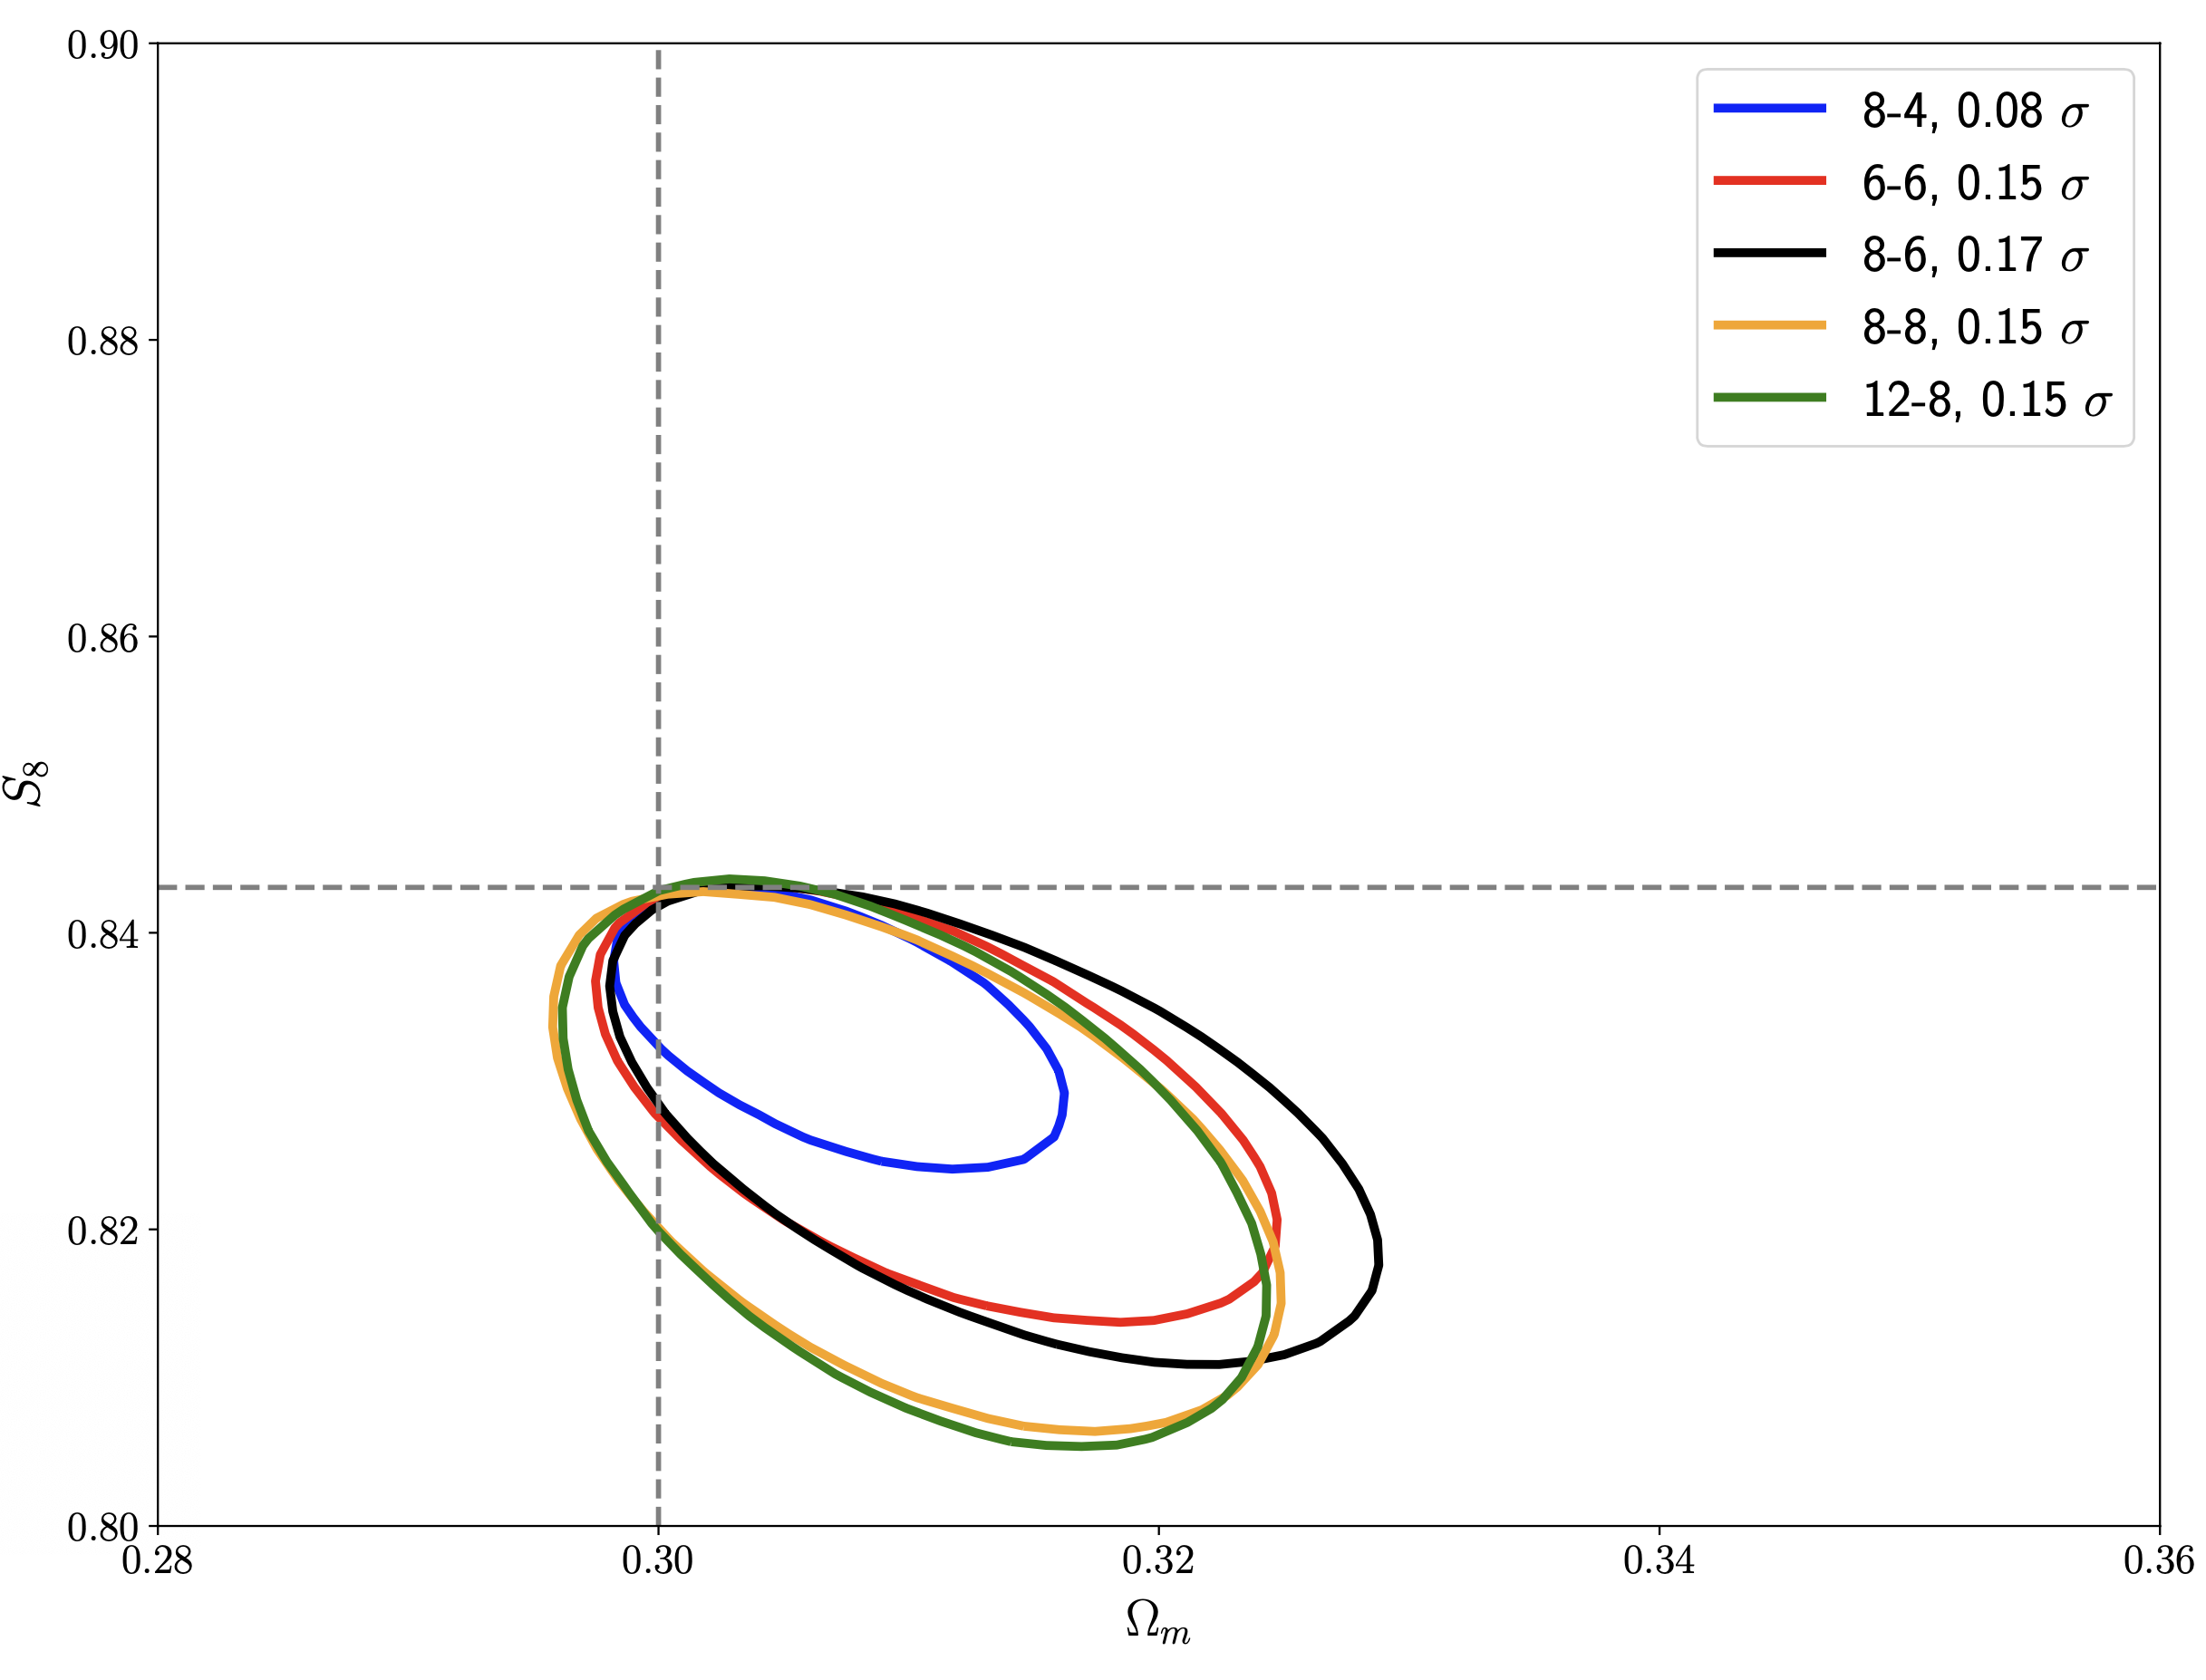
\includegraphics[width=\columnwidth,draft]{figs/temp.png}
\caption[]{Show the recovered bias values and the estimate from expected halo bias convolved with measured HOD from either small scales gglensing or in MICE. }
\label{fig:bias_relation}
\end{figure}


\section*{Acknowledgements}

The Acknowledgements section is not numbered. Here you can thank helpful
colleagues, acknowledge funding agencies, telescopes and facilities used etc.
Try to keep it short.

%%%%%%%%%%%%%%%%%%%%%%%%%%%%%%%%%%%%%%%%%%%%%%%%%%

%%%%%%%%%%%%%%%%%%%% REFERENCES %%%%%%%%%%%%%%%%%%

% The best way to enter references is to use BibTeX:

\bibliographystyle{mnras}
\bibliography{ref} % if your bibtex file is called example.bib


% Alternatively you could enter them by hand, like this:
% This method is tedious and prone to error if you have lots of references
% \begin{thebibliography}{99}
% \bibitem[\protect\citeauthoryear{Author}{2012}]{Author2012}
% Author A.~N., 2013, Journal of Improbable Astronomy, 1, 1
% \bibitem[\protect\citeauthoryear{Others}{2013}]{Others2013}
% Others S., 2012, Journal of Interesting Stuff, 17, 198
% \end{thebibliography}

%%%%%%%%%%%%%%%%%%%%%%%%%%%%%%%%%%%%%%%%%%%%%%%%%%

%%%%%%%%%%%%%%%%% APPENDICES %%%%%%%%%%%%%%%%%%%%%

\appendix

\section{2$\times$2pt Measurements}\label{app:2x2pt_measure}

\subsection{Point mass marginalization}
\begin{figure}
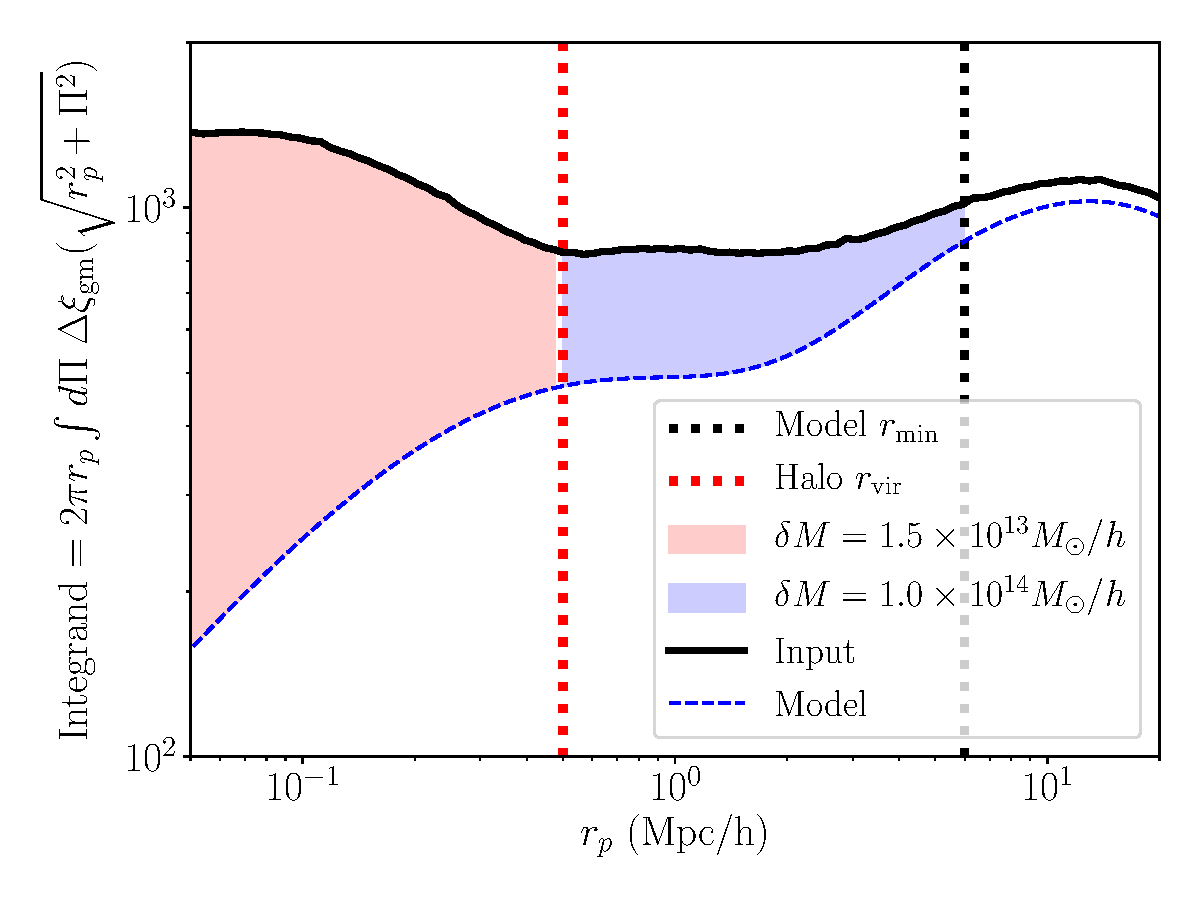
\includegraphics[width=\columnwidth]{figs/PM_contribution_radial.pdf}
\caption[]{We show the contribution of the PM to the galaxy-matter correlation in different radial regimes. The input is a halo-matter correlation function generated for a halo mass of $2.5 \times 10^{13} M_{\odot}/h$ using the NFW profile in the 1-halo regime ($r < 0.5 Mpc/h$) and 1Loop PT in the 2-halo regime ($r > 0.5 Mpc/h$). The model curve is generated from parameters within 1$\sigma$ of the truth. We show the contribution of the PM term separately for the 1-halo  and 2-halo regimes (up to the scale cut of 8Mpc/$h$). We find that the 2-halo regime contributes significantly. Therefore to put informative prior on the PM, the exact dependence of PM on cosmology and bias has to be known. 
}
\label{fig:pm_prior}
\end{figure}




\subsection{Model stress test}
\subsubsection{Evolution of Point-mass parameters}
The baseline model parameterization assumes the point mass parameter to be constant within each tomographic bin. We test this assumption by estimating the contribution that evolution of the galaxy-matter correlation function will have on the point mass parameters. Using a similar procedure as shown in Fig.~\ref{fig:pm_prior}, we estimate the integrand ($\delta_{\rm ev} M^{j}_{\rm halo}$) between evolved galaxy-matter correlation functions at edges of each tomographic bin $j$. These measured $\delta_{\rm ev} M^{j}_{\rm halo}$ quantify the expected bias in PM parameters due to evolution of the galaxy-matter correlations. These biases in PM parameters can potentially result in biased cosmology if it is a significant fraction of uncertainty in PM parameters ($\delta M^{j}_{\rm halo}$) for each tomographic bin $j$ (see Fig.~\ref{fig:pm_effect} for third tomographic bin) at our scale cuts. We compare the $\delta_{\rm ev} M^{j}_{\rm halo}$ to $\delta M^{j}_{\rm halo}$ in Fig.~\ref{fig:pm_evolve}. We see that for 2x2pt, the uncertainty in PM parameters is significantly greater than the expected bias. For 3x2pt, this bias is a significant fraction of the uncertainty but that will not bias our cosmology inference because as we have seen from Fig.~\ref{fig:pm_effect}, using shear information breaks the degeneracy between PM parameters and cosmological parameters.


\begin{figure}
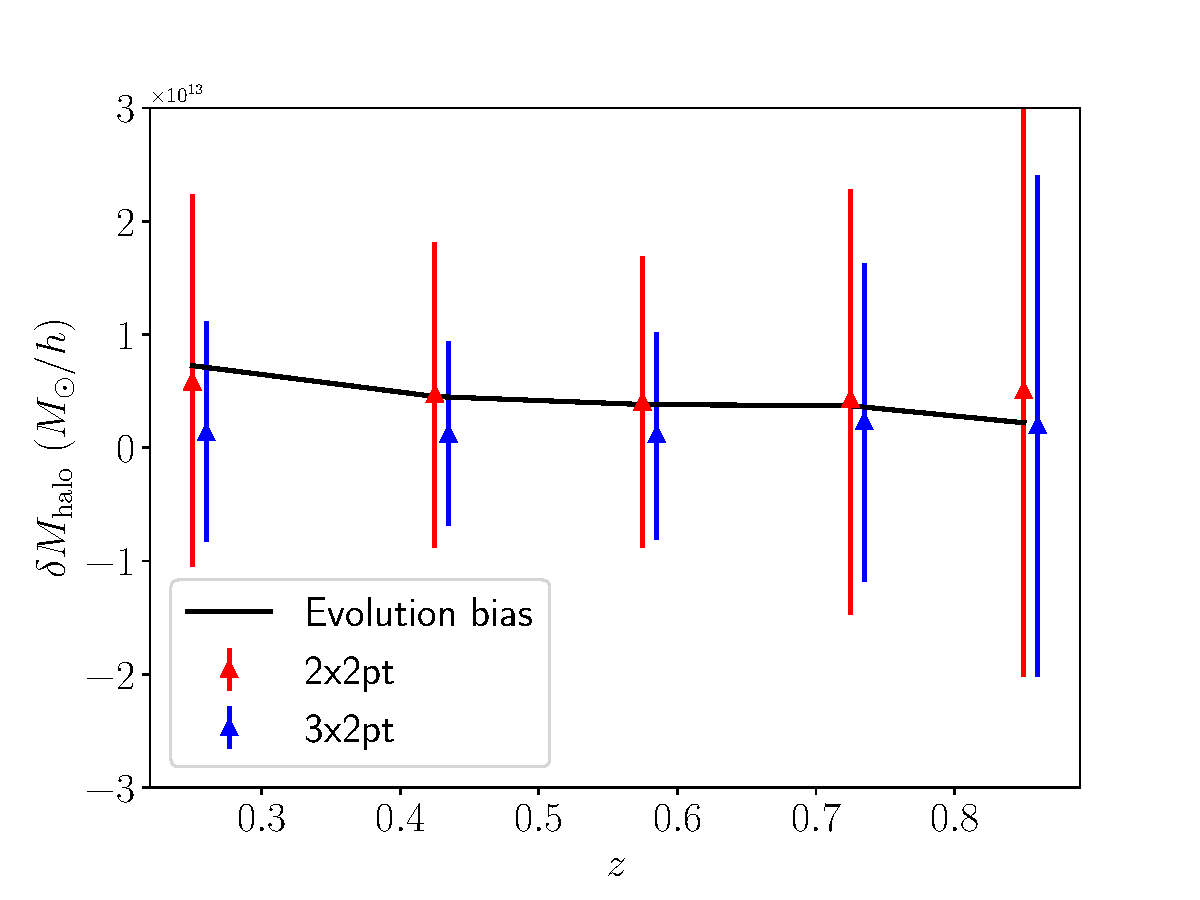
\includegraphics[width=\columnwidth]{figs/PM_evolve_impact.pdf}
\caption[]{We show the bias incurred from evolution of galaxy matter correlation on the PM parameters for each tomographic bin in black line. The red errorbars show the expected errorbars on PM parameters for 2x2pt as shown in Fig.~\ref{fig:pm_effect}. The blue errorbars are the constraints from 3x2pt. \SP{need to make this figure with non-zero PM values and at (8,6,0.5) scale cuts. It seems the impact will be even smaller there probably.}
}
\label{fig:pm_evolve}
\end{figure}




\subsection{Simulations}

\begin{figure}
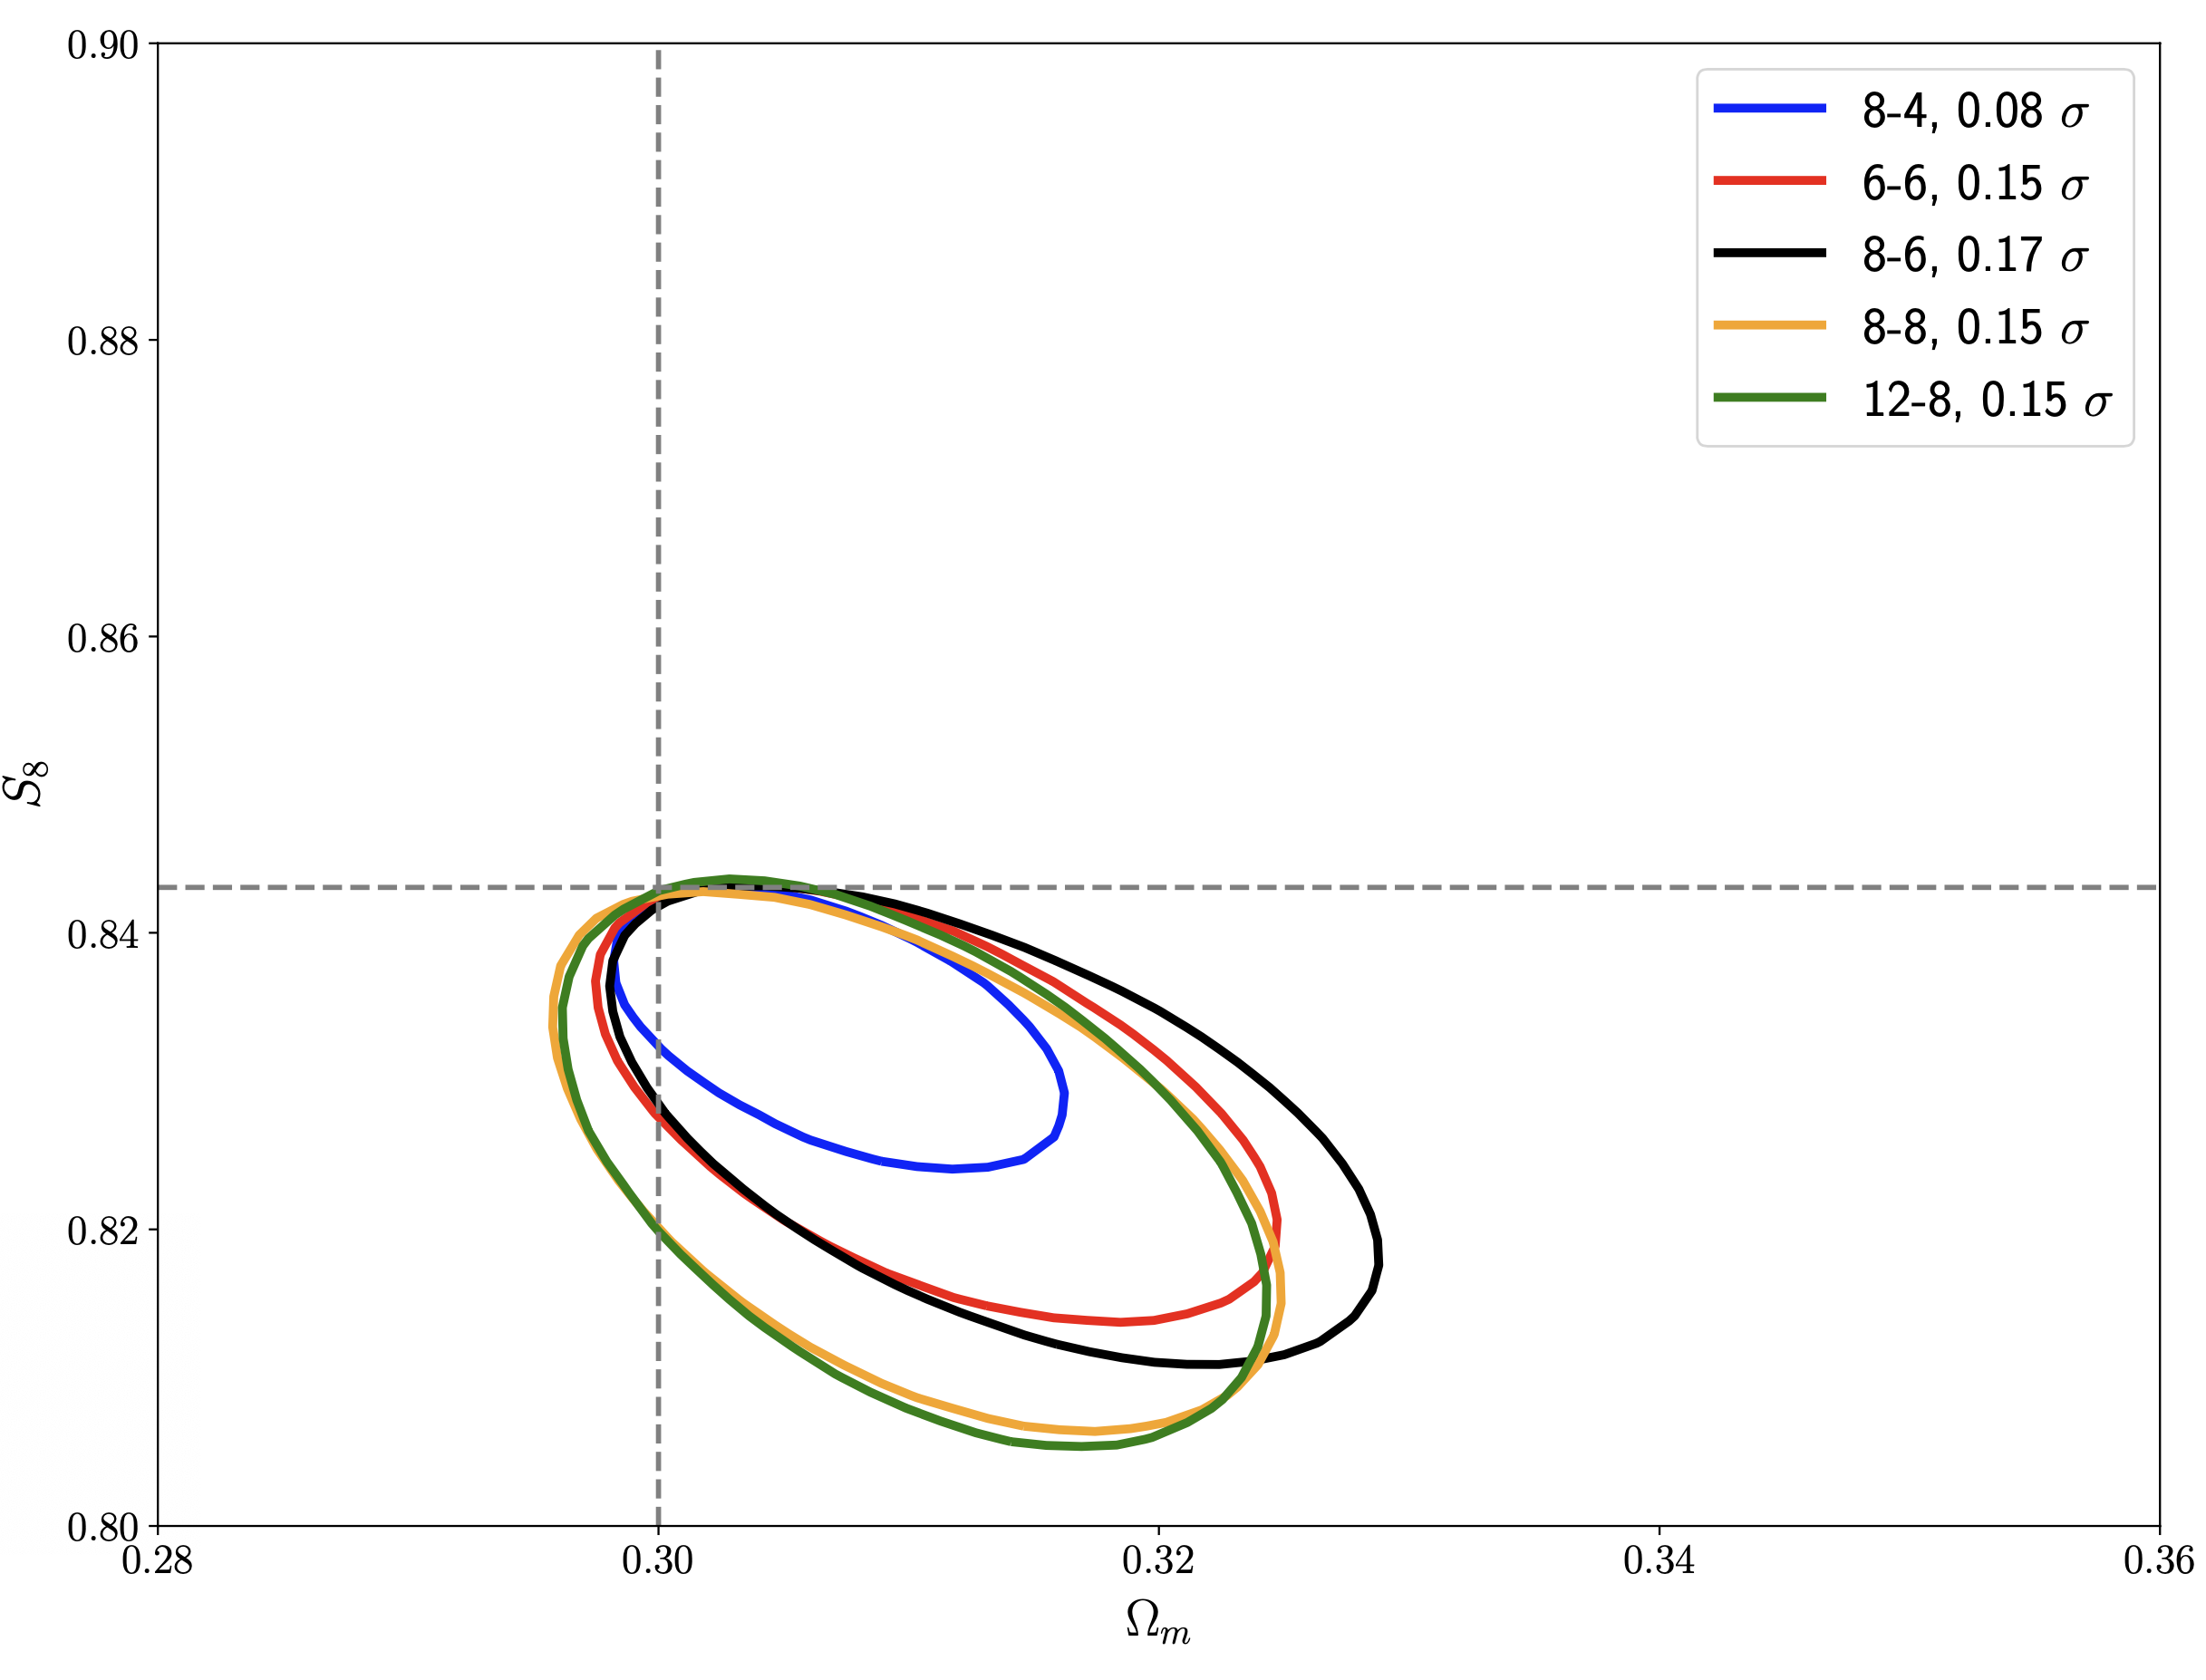
\includegraphics[width=0.5\textwidth,draft]{figs/temp.png}
\caption[]{Measurements of \wtheta and \gammat for \buzzard \ simulations. Show results for mean of N realizations and bestfit theory }
\label{fig:buzzard_2pt}
\end{figure}

\begin{figure}
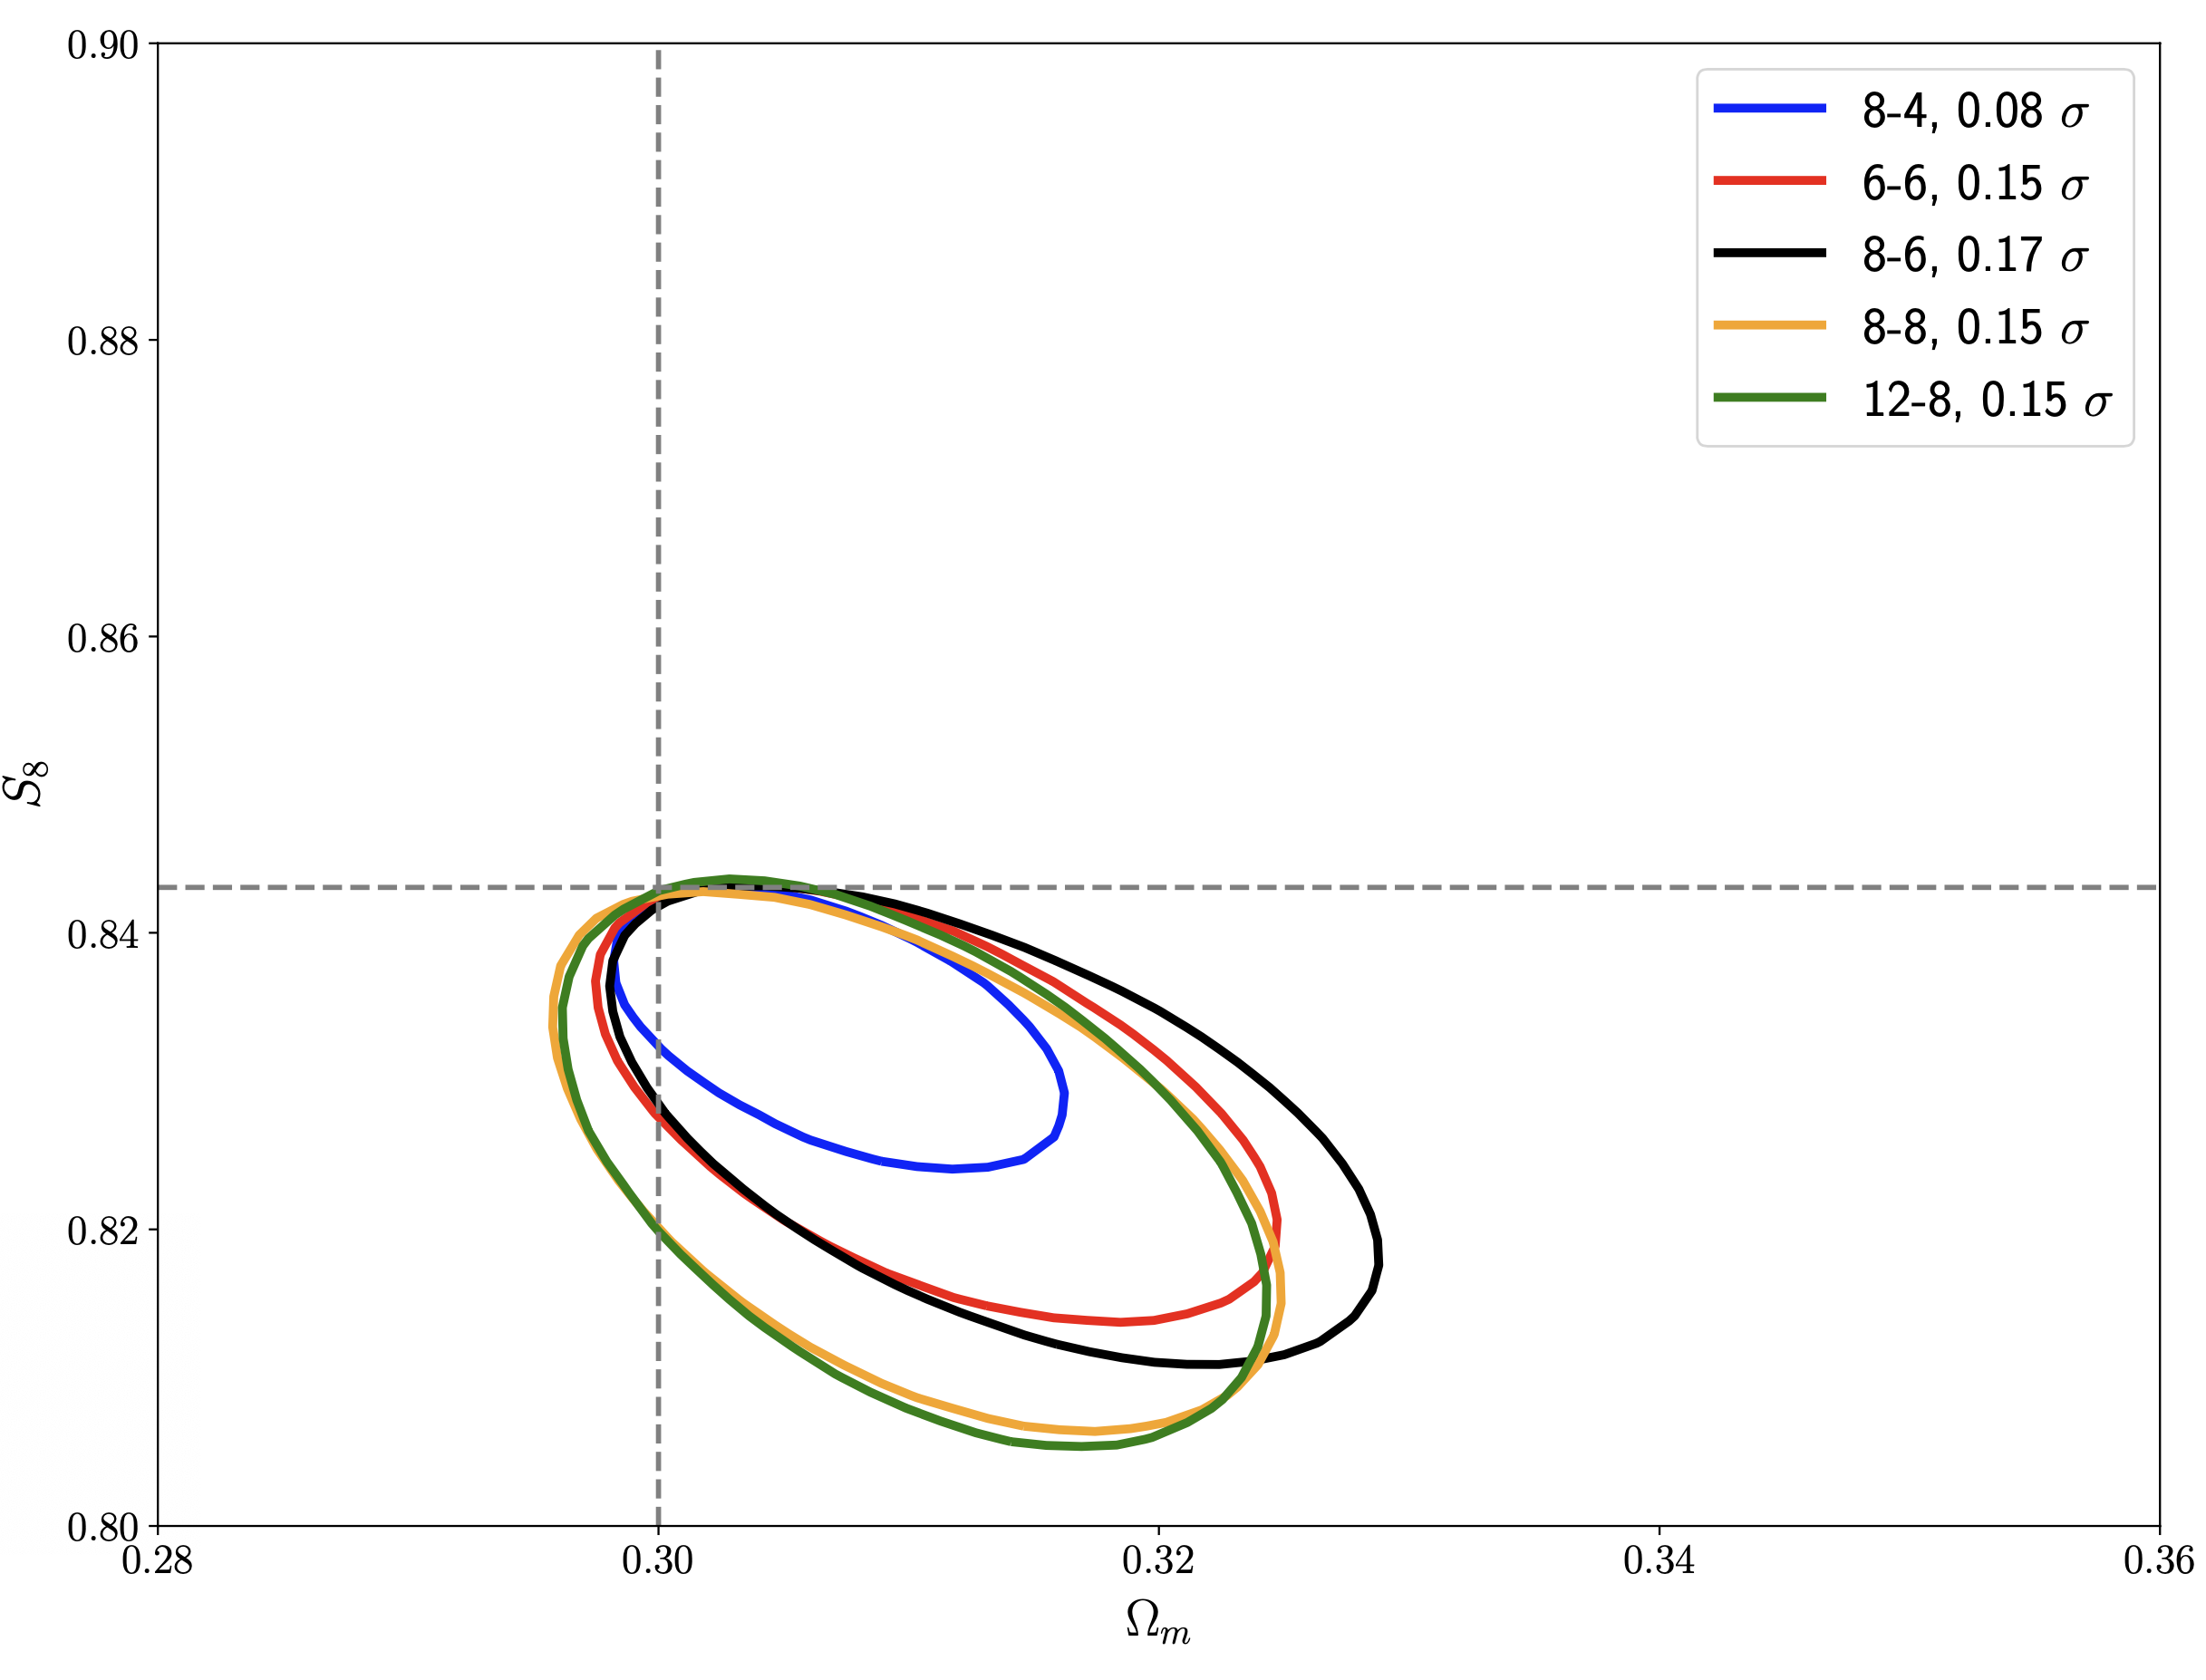
\includegraphics[width=0.5\textwidth,draft]{figs/temp.png}
\caption[]{Measurements of \wtheta and \gammat for \mice \  simulations }
\label{fig:mice_2pt}
\end{figure}

\subsection{DES Y3}
\begin{figure}
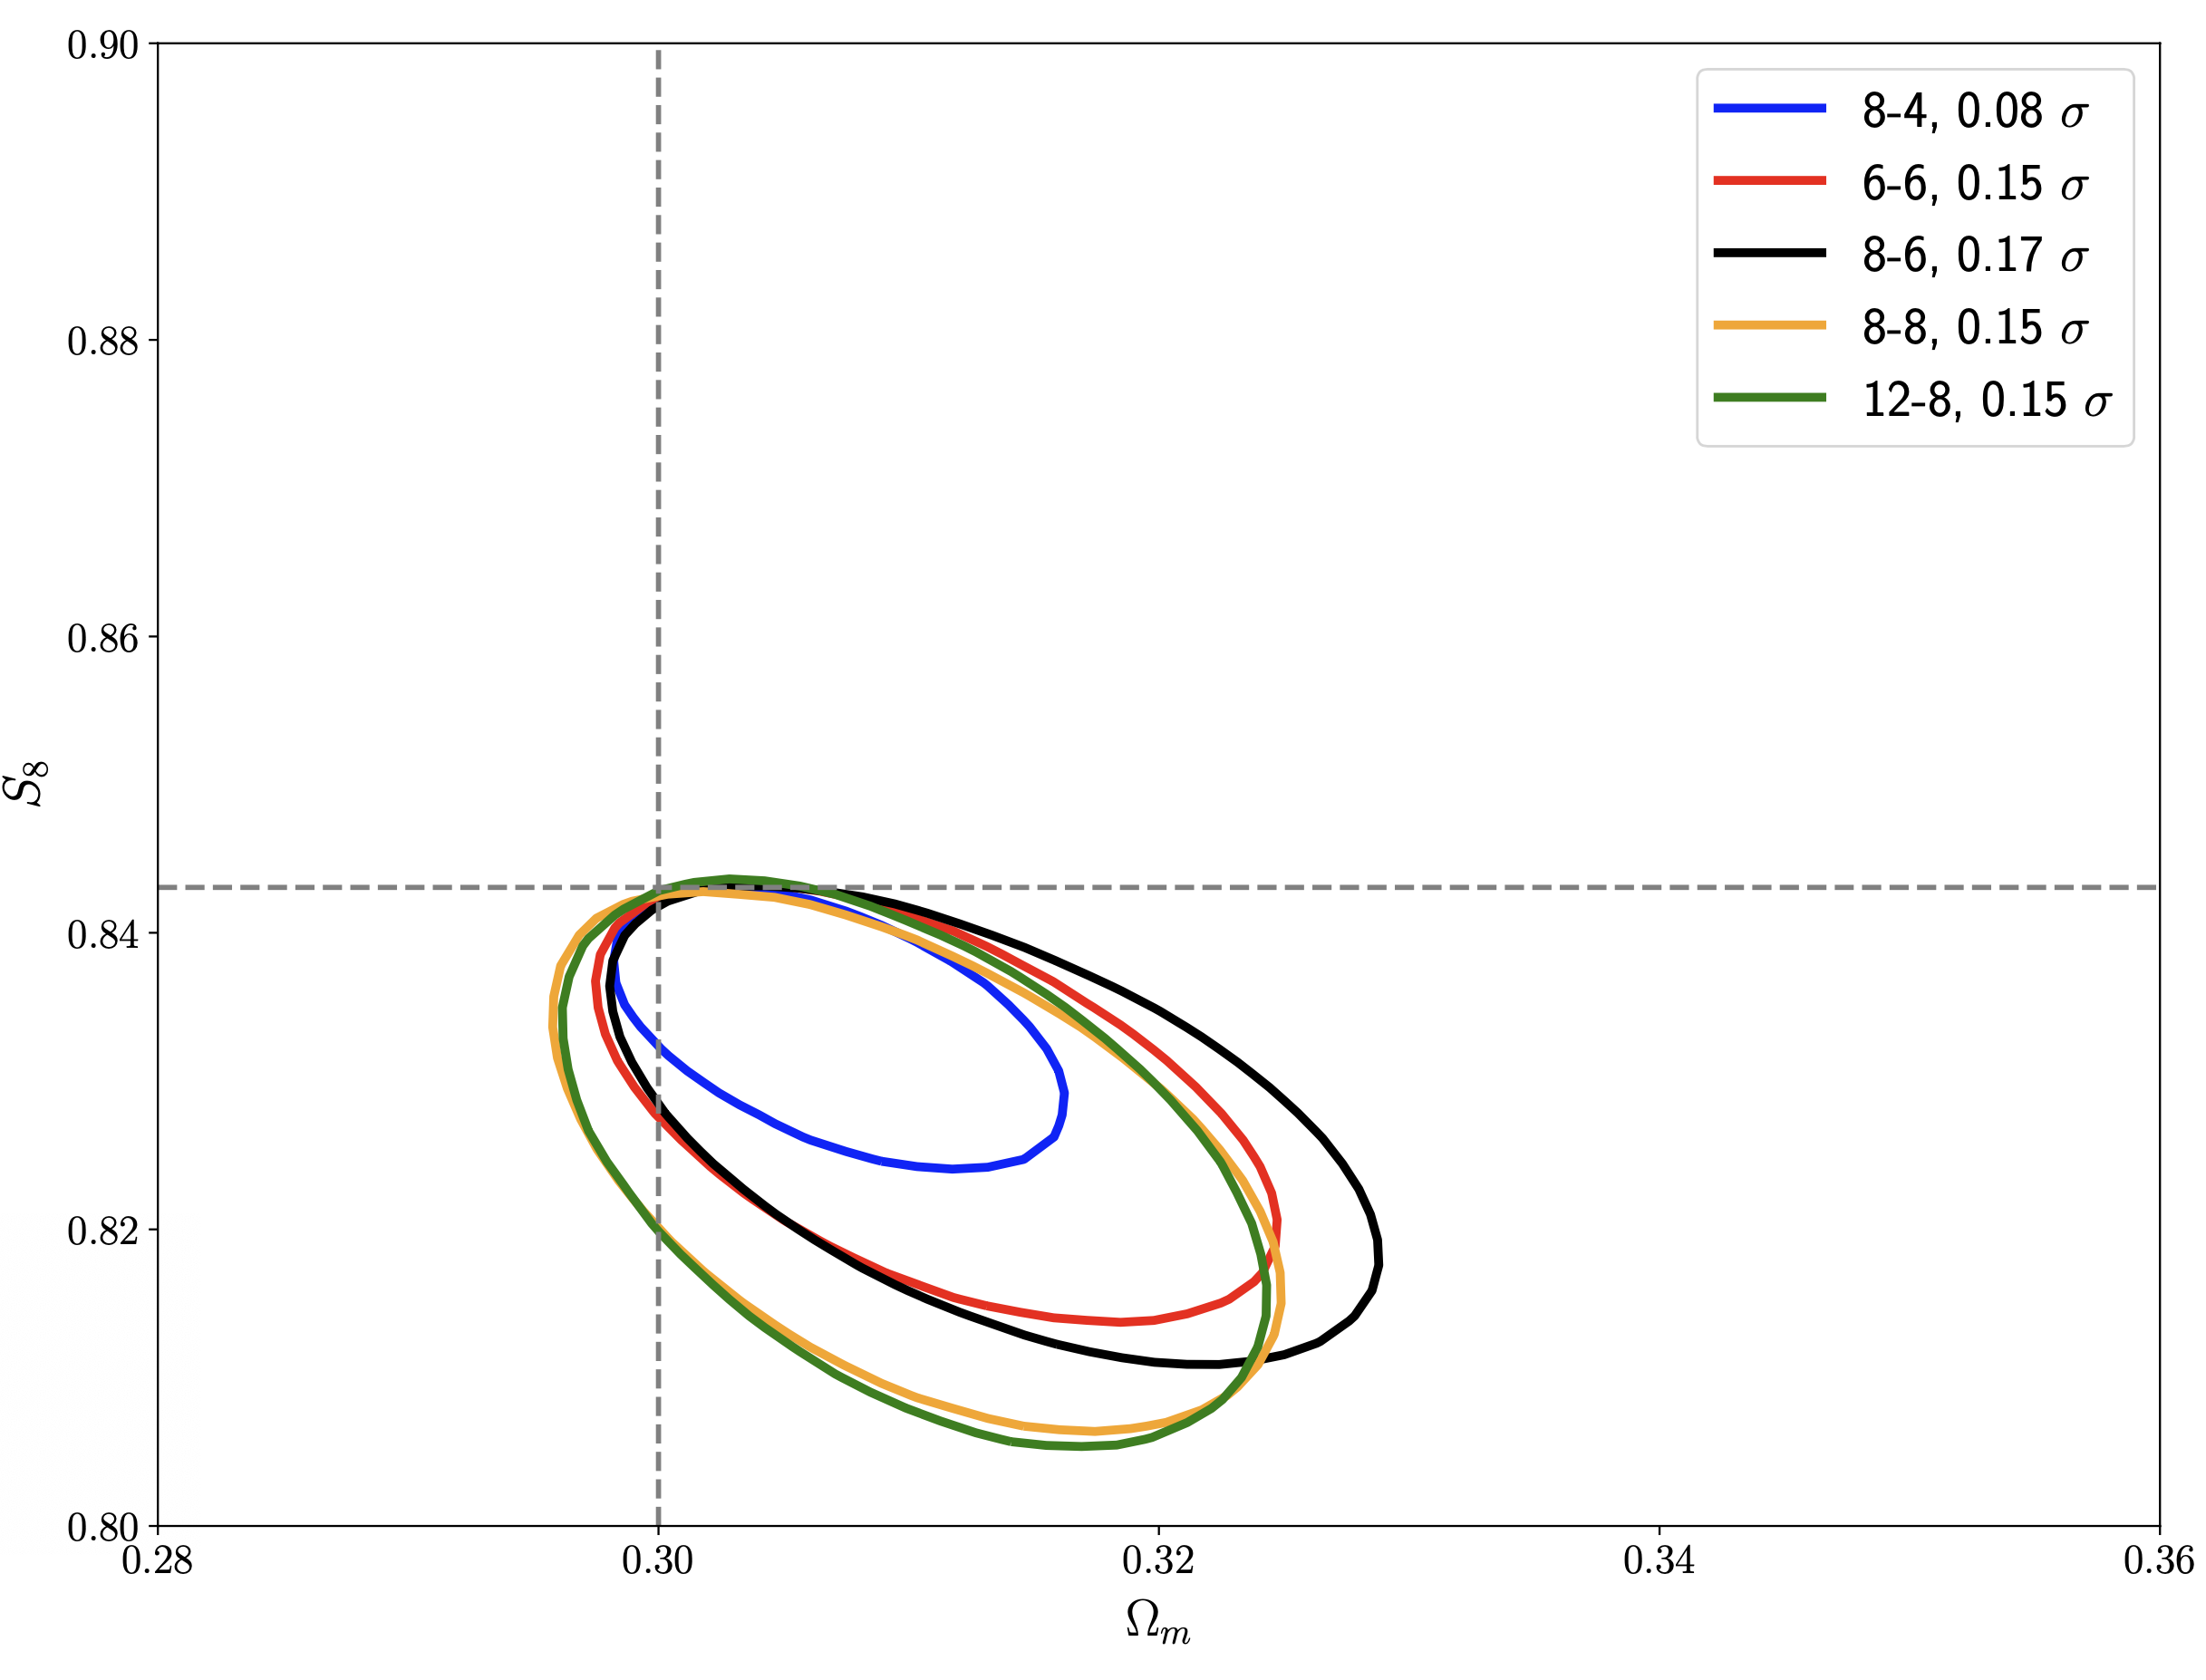
\includegraphics[width=0.5\textwidth,draft]{figs/temp.png}
\caption[]{Measurements of \wtheta and \gammat for DES Y3 data }
\label{fig:data_2pt}
\end{figure}

\section{Scale cuts validation}\label{app:scale_cuts}
\subsection{Projection effects}\label{app:projection_effects}

\begin{figure}
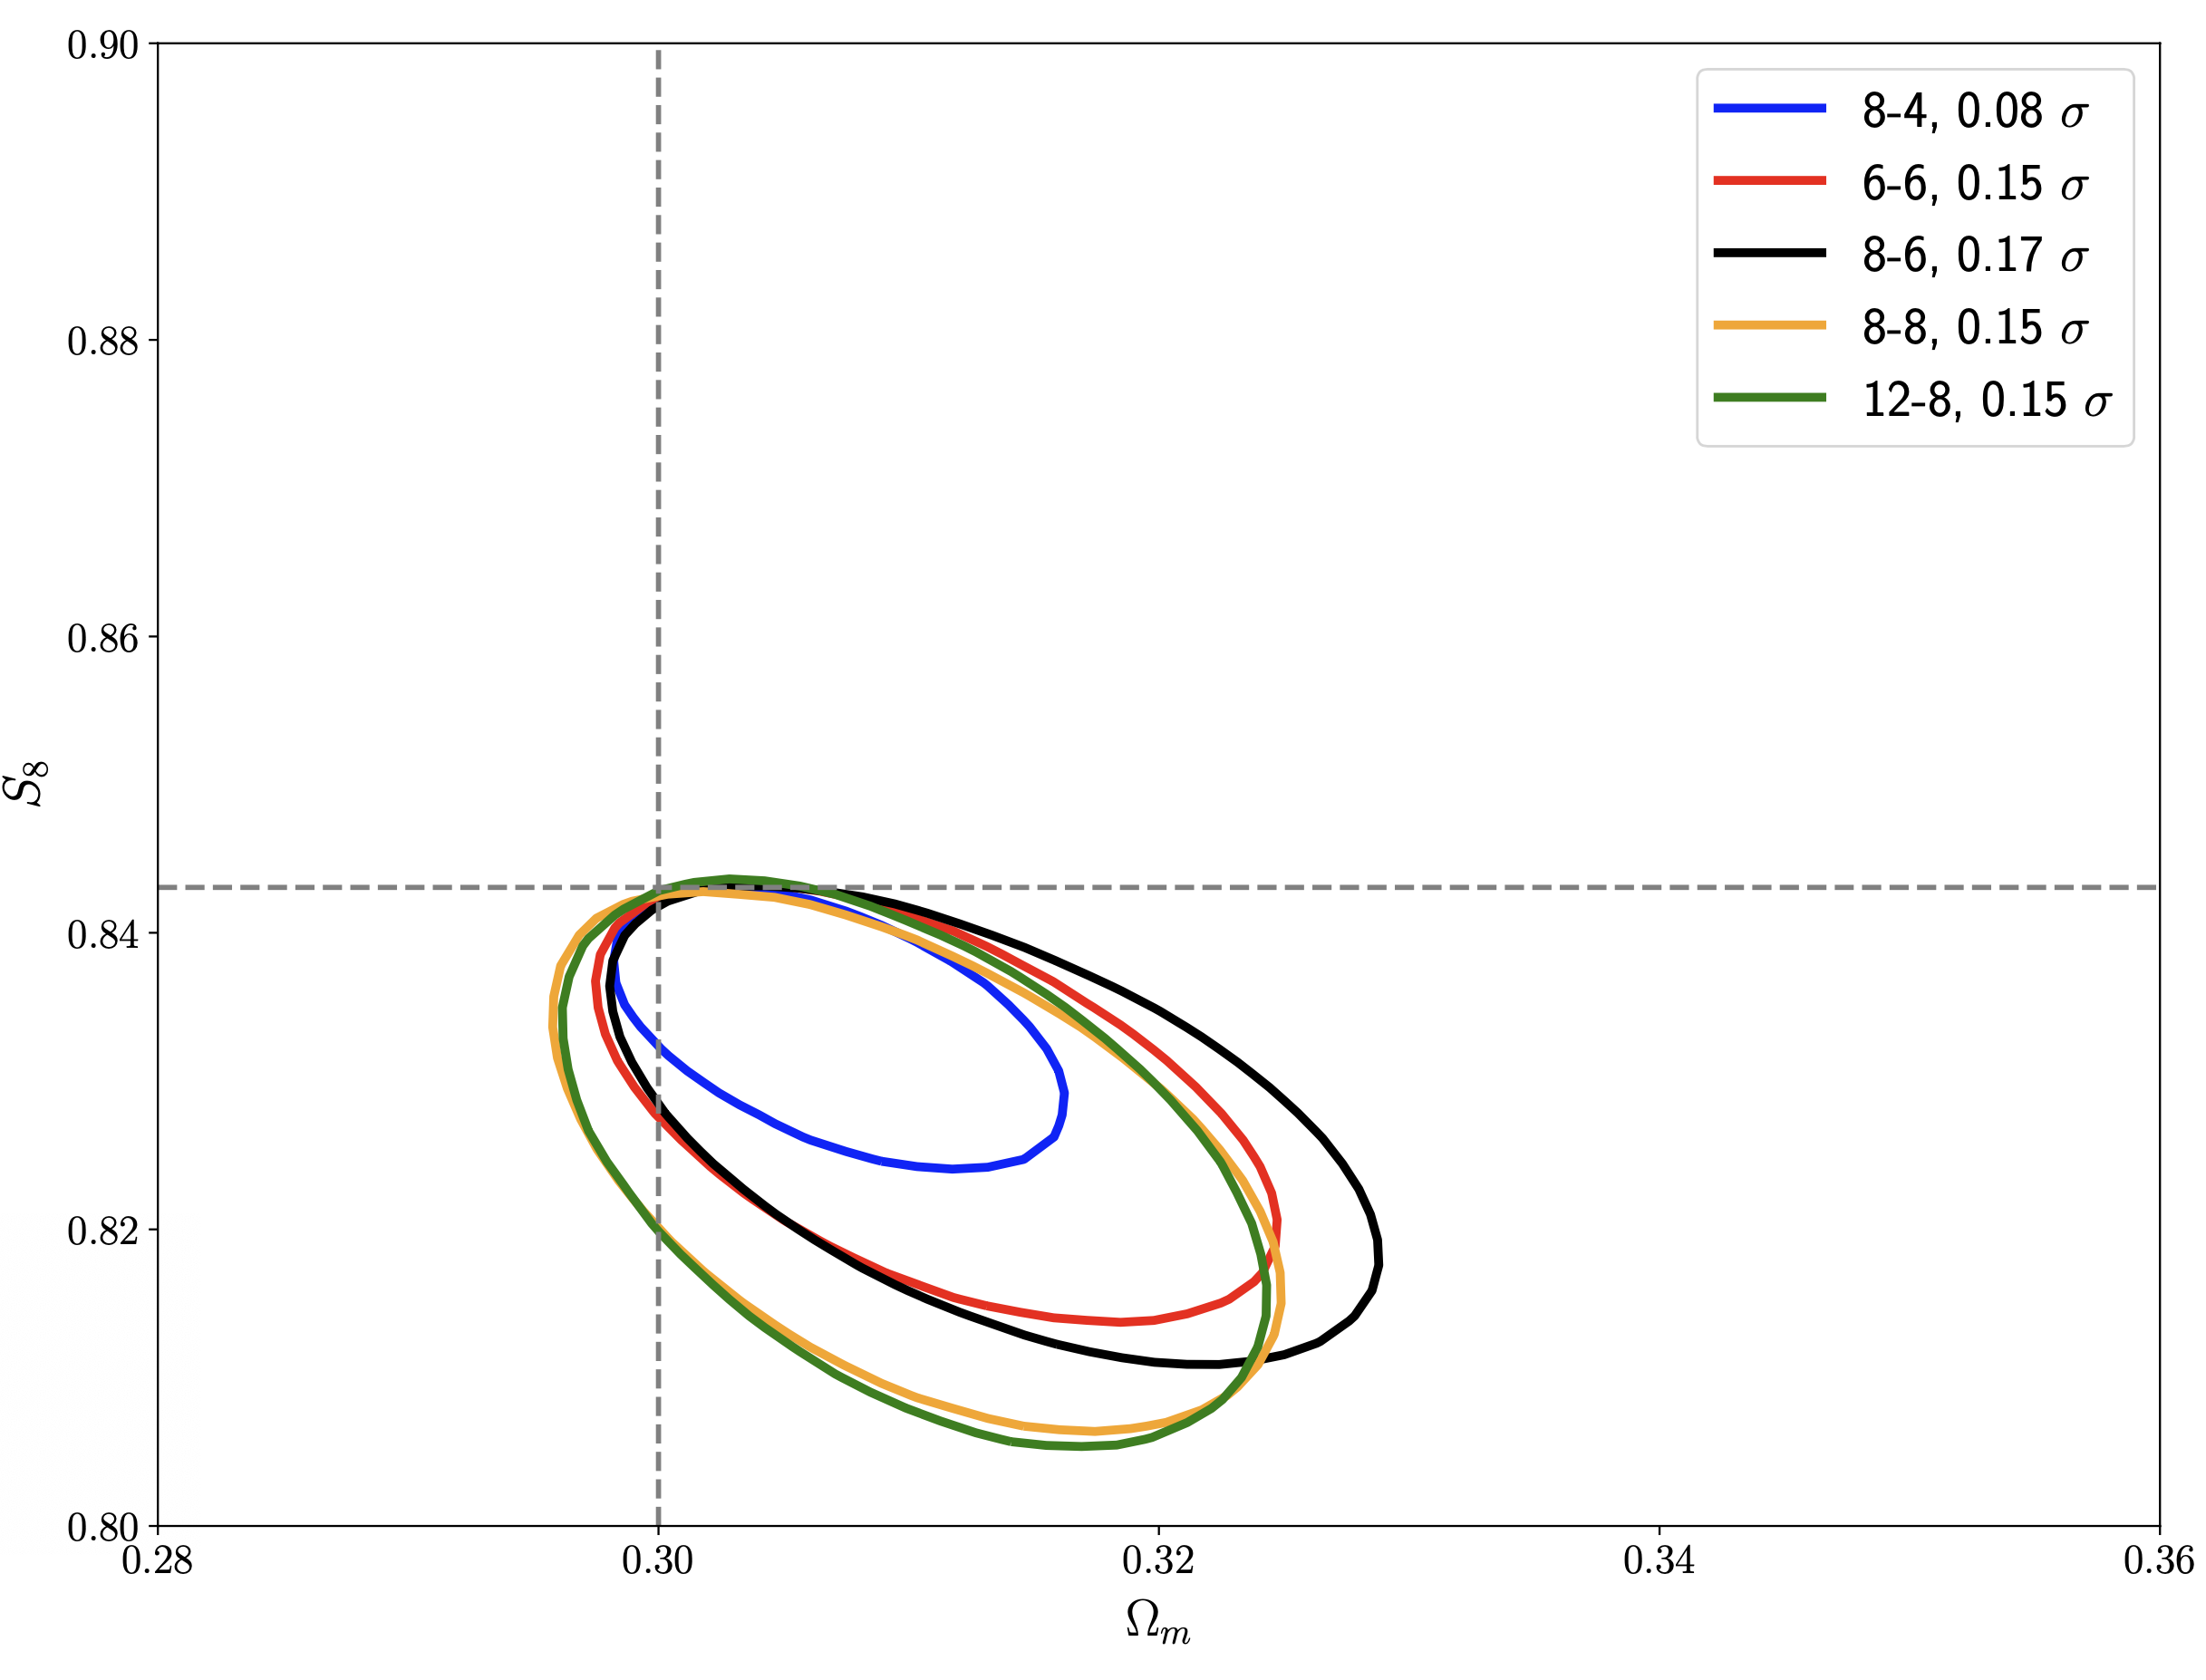
\includegraphics[width=0.5\textwidth,draft]{figs/temp.png}
\caption[]{Show profile likelihood plots to show that we recover correct likelihood for cosmology parameters, while the posteriors are biased}
\label{fig:prof_like}
\end{figure}

\begin{figure*}
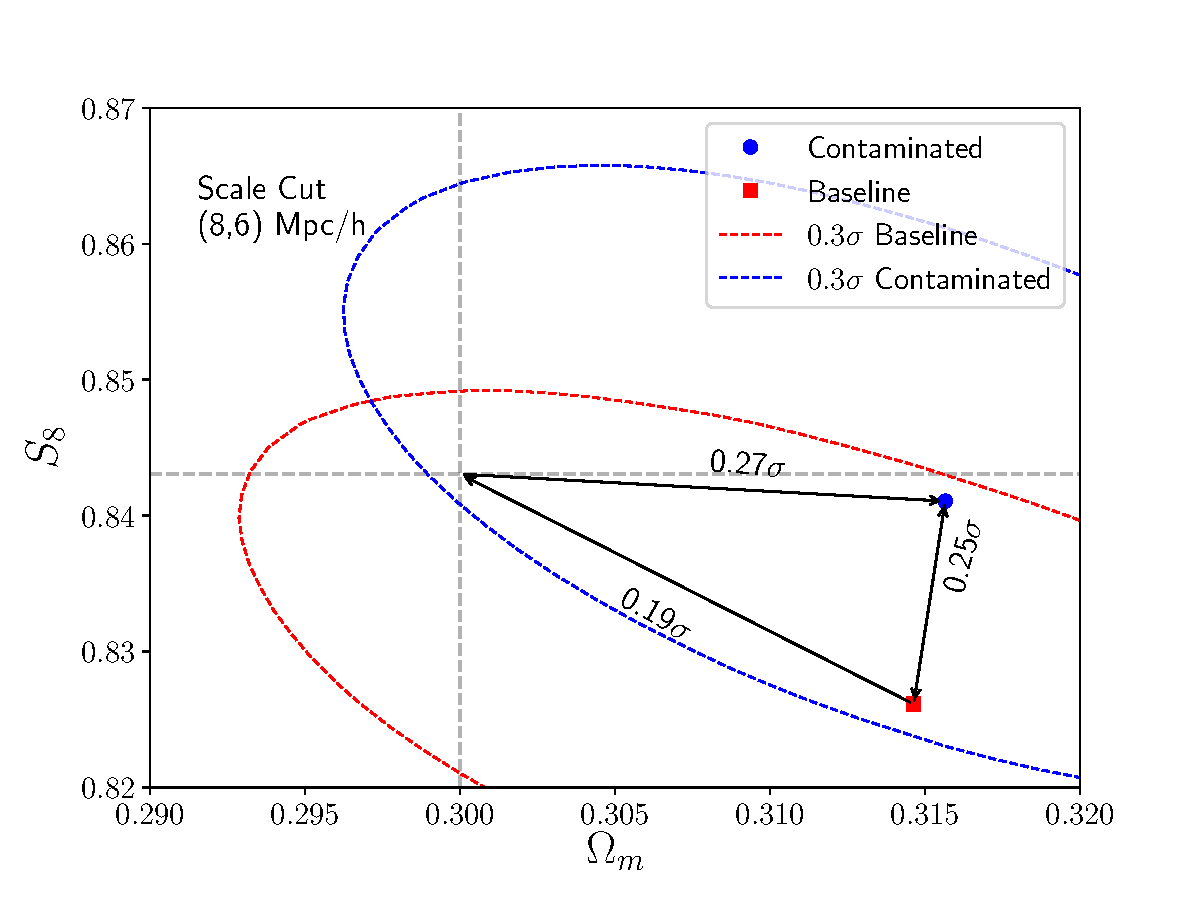
\includegraphics[width=\columnwidth]{figs/contour_2x2pt_sc_8_6.pdf}
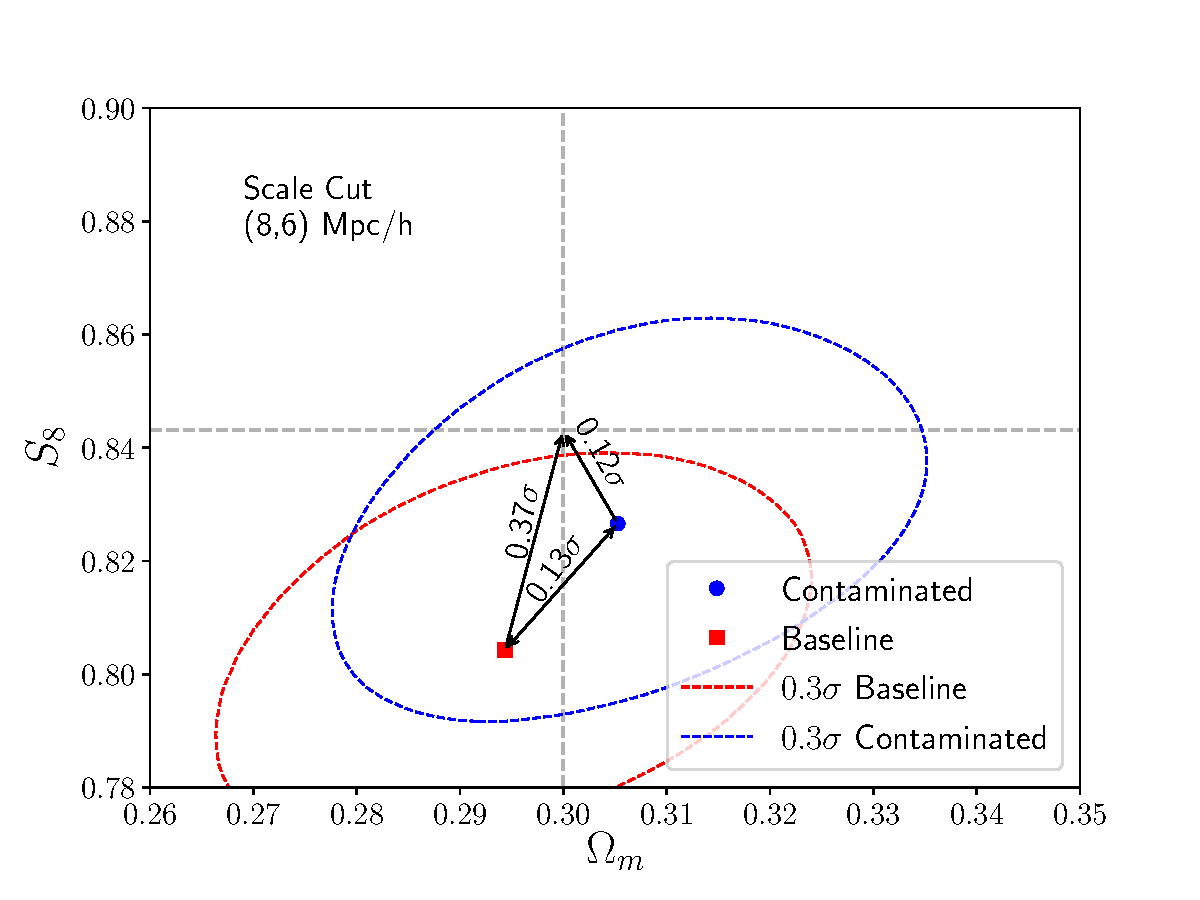
\includegraphics[width=\columnwidth]{figs/contour_2x2pt_sc_8_6_wcdm.pdf}
\caption[]{Show the contour plots and biases in cosmology in the 2D space. Left is for $\Lambda$CDM and right is for $w$CDM. Show that the projection effects are much smaller in the 2D space}
\label{fig:2d_simlike}
\end{figure*}

\begin{figure}
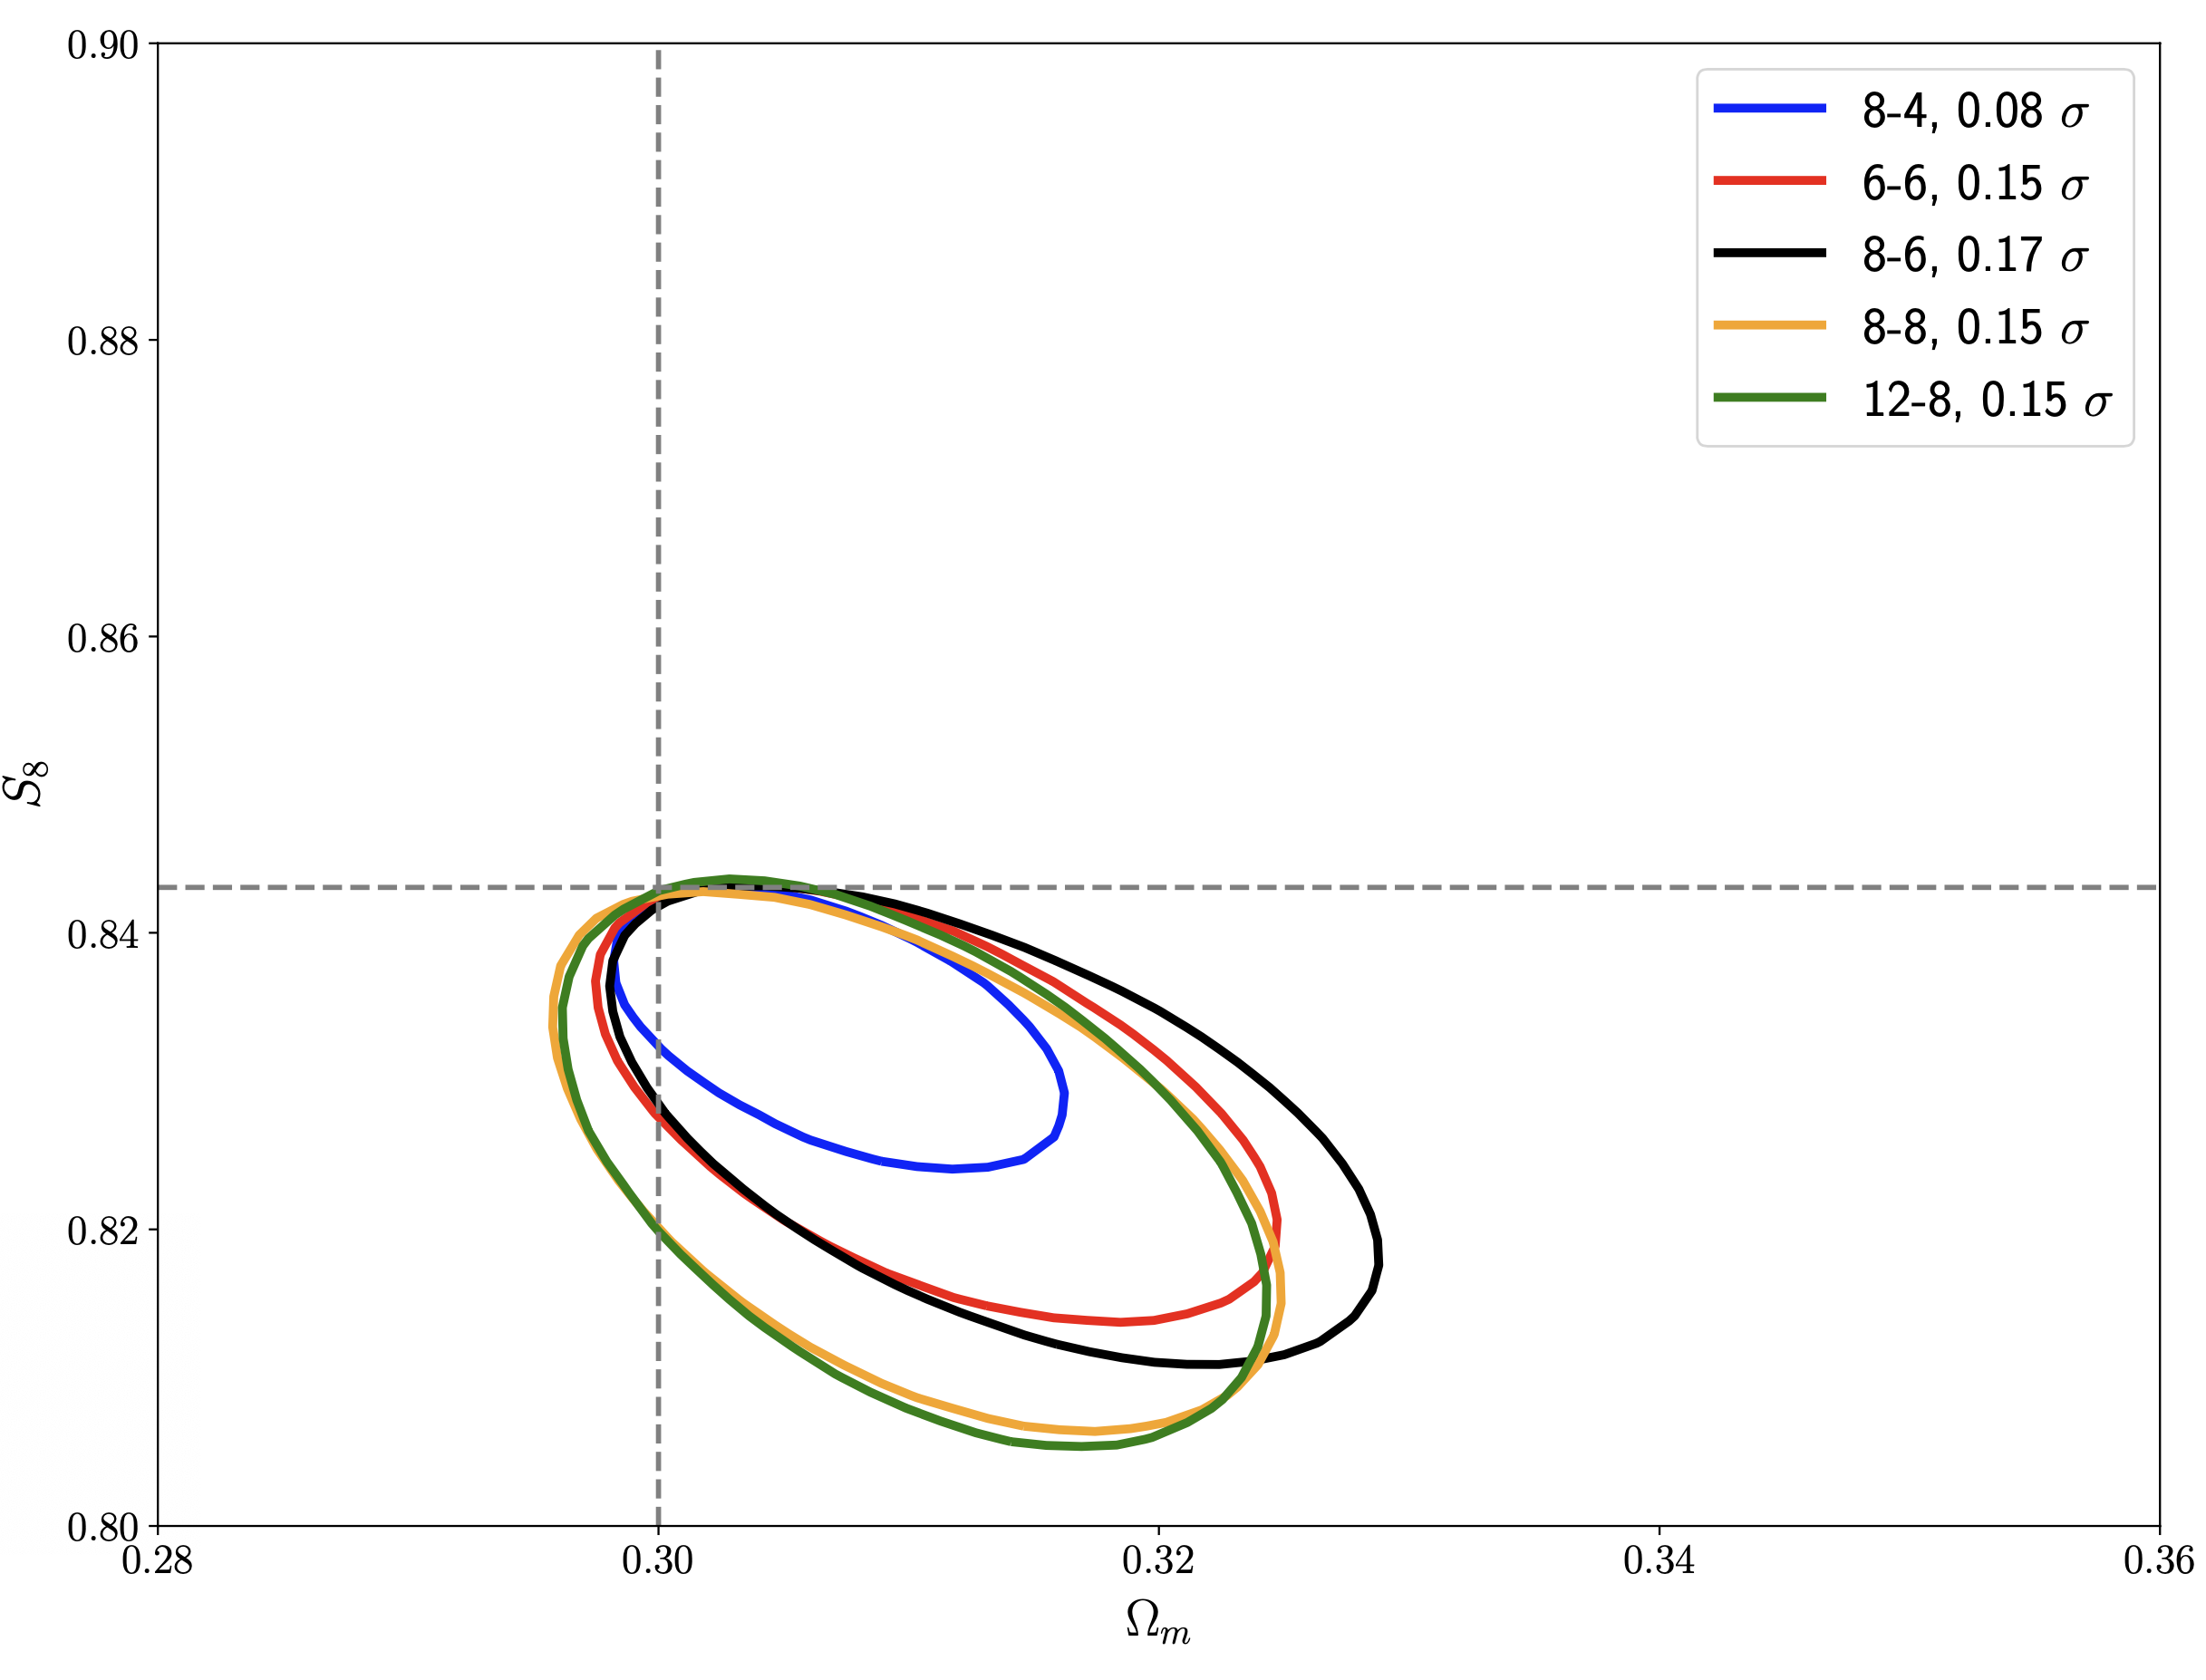
\includegraphics[width=0.5\textwidth,draft]{figs/temp.png}
\caption[]{Show that the projection effects are smaller when using the prior set (ii), i.e. informative priors on $\theta_{\star}$, $\Omega_{\rm b} h^2$ and $n_s$.}
\label{fig:simlike_cosmoprior}
\end{figure}



%%%%%%%%%%%%%%%%%%%%%%%%%%%%%%%%%%%%%%%%%%%%%%%%%%


% Don't change these lines
\bsp	% typesetting comment
\label{lastpage}

% \bibliographystyle{apsrev4-1}
% \bibliography{ref} 

\end{document}

% End of mnras_template.tex